% This example is meant to be compiled with lualatex or xelatex
% The theme itself also supports pdflatex
\PassOptionsToPackage{unicode}{hyperref}
\documentclass[aspectratio=1610, 9pt]{beamer}

% Load packages you need here
\usepackage{polyglossia}
\setmainlanguage{german}

\usepackage{csquotes}
    

\usepackage{amsmath}
\usepackage{amssymb}
\usepackage{mathtools}

\usepackage{hyperref}
\usepackage{bookmark}

% load the theme after all packages

\usetheme[
  showtotalframes, % show total number of frames in the footline
]{tudo}

% Put settings here, like
\unimathsetup{
  math-style=ISO,
  bold-style=ISO,
  nabla=upright,
  partial=upright,
  mathrm=sym,
}

\usepackage[%%%%%%%%%%%%%%%%%%%%%%%%%%%%%%%%%%%%%%%%%%%by RK
  locale=DE,
  separate-uncertainty=true,
  per-mode=symbol-or-fraction,
]{siunitx}
\sisetup{math-micro=\text{µ},text-micro=µ}

\title{Temperaturabhängigkeit der
magnetisch kontrollierten direktionalen
Lichtemission in plasmonischen
Halbleiter-Hybridstrukturen}
\author[R.~Kaiser]{Raphael Kaiser}
\institute[Experimentelle Physik II]{Experimentelle Physik II \\ Fakultät Physik}
%\titlegraphic{\includegraphics[width=0.7\textwidth]{images/tudo-title-2.jpg}}


\begin{document}

\maketitle

\begin{frame}{Inhaltsverzeichnis}
  \tableofcontents
\end{frame}

% hier werden die tex-files aus content eingefügt
%#############################
%####MUSTER FÜR EINE FOLIE####   
%#############################

%\begin{frame}{titel}
%    \pause
%    \begin{columns}
%        \begin{column}{0.5\textwidth}
%            \begin{itemize}
%                \item <->
%                \item <->
%                \item <->
%                \item <->
%                \item <->
%                \item <->
%            \end{itemize}
%        \end{column}
%        \begin{column}{0.5\textwidth}
%            \centering
%            \only <->{
%                \includegraphics[scale=0.25]{images/}\\[-0.5\baselineskip]
%                \hspace{1.5cm}}%\href{www. ...}{[name, paper]}
%             }
%        \end{column}
%    \end{columns}
%\end{frame}

\begin{frame}{Einleitung}
    \pause
    \begin{columns}
        \begin{column}{0.5\textwidth}
            \begin{itemize}
                \item <1-> magnetooptische Effekte \leftrightarrow Zusammenspiel zwischen Licht, Materie und magnetischen Feldern
                    \begin{itemize}
                        \item <2-> z.B. Faraday Effekt (1845)
                        \item <3-> TMOKE
                    \end{itemize}
                \bigskip 
                \item <4-> heute \rightarrow TMRLE 
                    \begin{itemize}
                        \item <5-> Effekte klein \rightarrow Verstärkung durch plasmonische Strukturen
                    \end{itemize}
                \bigskip 
                \item <6-> Warum das Ganze?
                \item <7-> mögliche technische Nutzbarkeit \rightarrow bessere Erforschung notwendig 
                \item <8-> Untersuchung der Temperaturabhängigkeit    
            \end{itemize}
        \end{column}
        \begin{column}{0.5\textwidth}
            \centering
            \only <2>{%
                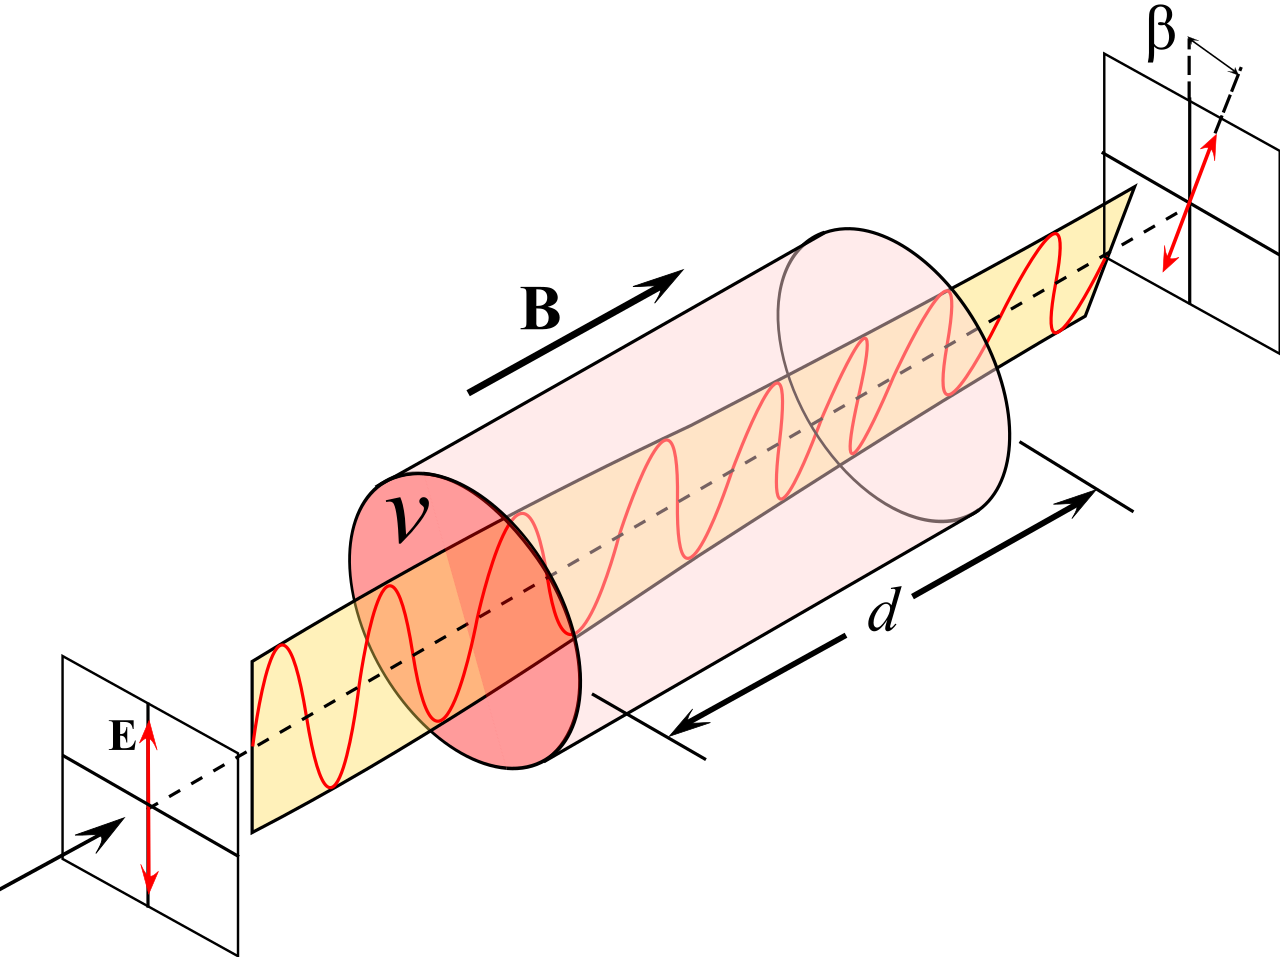
\includegraphics[scale=0.1]{images/faraday.png}\\[-1.5\baselineskip]%
                \hspace{1.5cm}{[JunCTionS, Wikipedia]}}%
            \only <3>{%
                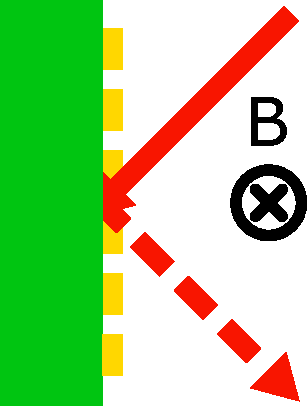
\includegraphics[scale=0.4]{images/TMOKE.pdf}\\[-0.5\baselineskip]%
                \hspace{1.5cm}{[Lars Klompmaker, Masterarbeit]}}%
            \only <4->{%
                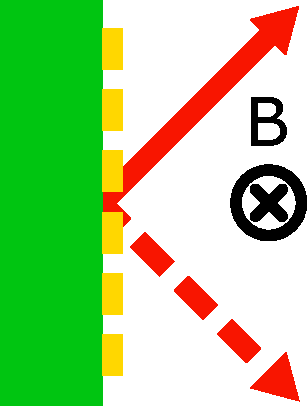
\includegraphics[scale=0.4]{images/TMRLE.pdf}\\[-0.5\baselineskip]%
                \hspace{1.5cm}{[Lars Klompmaker, Masterarbeit]}}%      
        \end{column}
    \end{columns}
\end{frame}
%#############################
%####MUSTER FÜR EINE FOLIE####   
%#############################

%\begin{frame}{titel}
%    \pause
%    \begin{columns}
%        \begin{column}{0.5\textwidth}
%            \begin{itemize}
%                \item <->
%                \item <->
%                \item <->
%                \item <->
%                \item <->
%                \item <->
%            \end{itemize}
%        \end{column}
%        \begin{column}{0.5\textwidth}
%            \centering
%            \only <->{
%                \includegraphics[scale=0.25]{images/}\\[-0.5\baselineskip]
%                \hspace{1.5cm}}%\href{www. ...}{[name, paper]}
%             }
%        \end{column}
%    \end{columns}
%\end{frame}


\section{Theoretische Erläuterungen}
%pause für pop effekt
%\subsection{Oberflächenplasmon-Polariton}
\begin{frame}{Oberflächenplasmon-Polariton}
    \pause
    \begin{columns}
    \begin{column}{0.5\textwidth}        
        \begin{itemize}
            %\item[\textbf{\textcolor{tugreen}{\to}}] lol
            \item <1-> kollektive Oszillationen des Elektronengases entlang einer Grenzfläche zwischen Leiter und Dielektrikum
            \bigskip   
            \item <3-> Plasmonen = Quasiteilchen
            \bigskip   
            \item <4-> theoretischer Zugang über Maxwell Gleichungen %\rightarrow $\nabla^2 \vec{E} + k^2_0 \, \epsilon \, \vec{E} = 0$
                \begin{itemize}
                    \item Plasmonen sind TM-Wellen
                \end{itemize}
            \bigskip            
            \item <5-> Dispersionsrelation $k_\text{spp} = k_0 \sqrt{\frac{\epsilon_1 \,\epsilon_2}{\epsilon_1 + \epsilon_2}}$
        \end{itemize}
    \end{column}
    \begin{column}{0.5\textwidth}
        \centering
        \only <2->{
            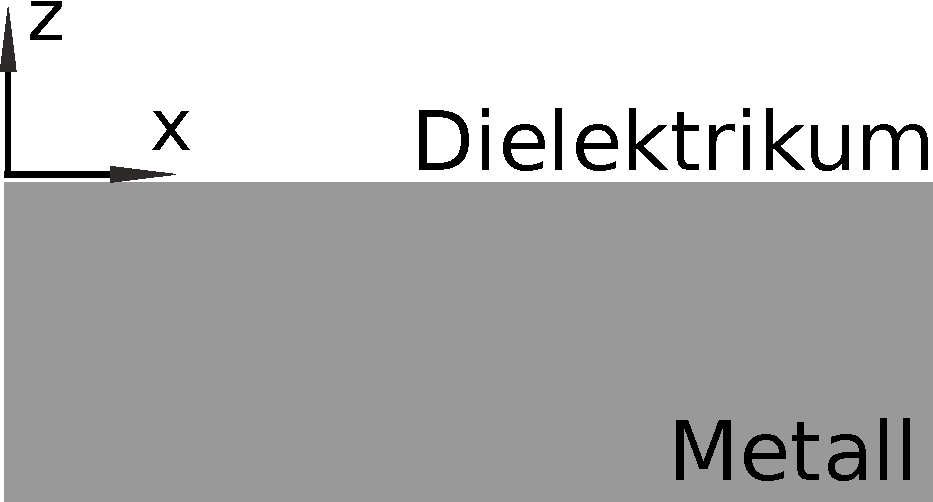
\includegraphics[scale=0.25]{images/leiter_und_nichtleiter.pdf}\\[-0.5\baselineskip]
            \hspace{1.5cm}}%        
    \end{column}        
    \end{columns}
\end{frame}

\begin{frame}{Oberflächenplasmon-Polariton}
    \begin{columns}
        \begin{column}{0.5\textwidth}
            \begin{itemize}
                \item <1-> Plasmonen lassen sich mit Licht anregen
                \bigskip
                \item <2-> Dispersionsrelation $k_\text{spp} = k_0 \sqrt{\frac{\epsilon_1 \,\epsilon_2}{\epsilon_1 + \epsilon_2}}$
                %\bigskip 
                \item <4-> Schnittpunkt: Energie- \& Impulserhaltung \rightarrow hier nicht \rightarrow keine Anregung
                \bigskip 
                \item <5-> Bedingung? \rightarrow Goldgitter auf Oberfläche nötig
                %\bigskip 
                \item <7-> $k_\text{SPP} = k \sin(\theta) \pm m \, G $ mit $m \in \mathbb{N}^+$ und $G = \frac{2 \, \pi}{a}$
               \bigskip 
                \item <8-> Prozess auch umgekehrt möglich. Plasmon kann als Licht auskoppeln.
            \end{itemize}
        \end{column}
        \begin{column}{0.5\textwidth}
            \centering
            \only <3->{
            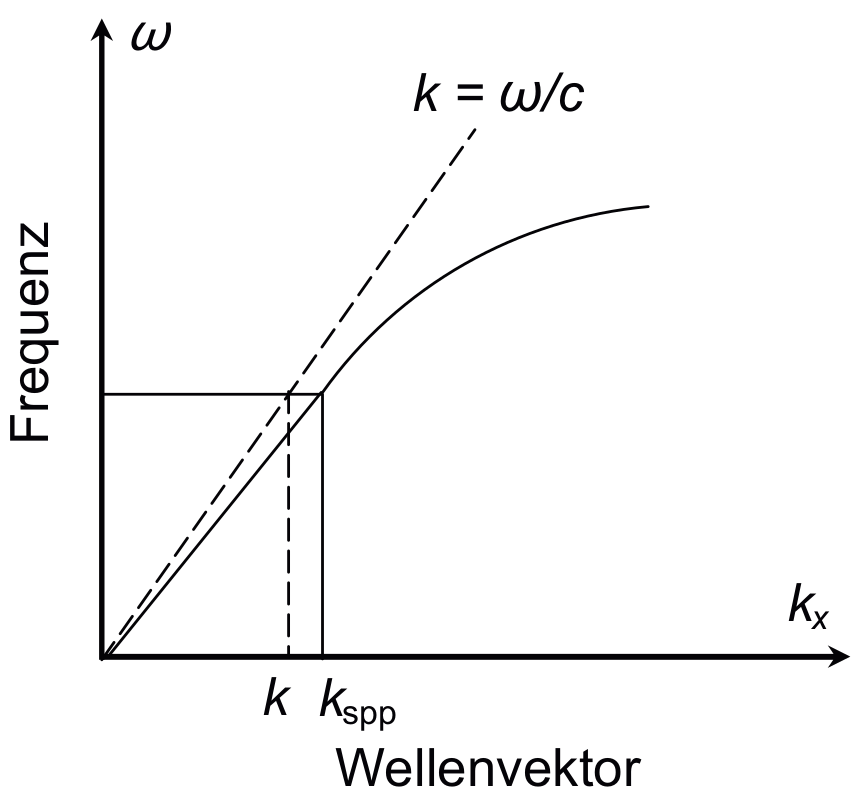
\includegraphics[width=3.5cm]{images/disp.png}\\ \hspace{1.5cm} {[{Stefan Maier, Plasmonics}]}
            }
            \only <6->{
            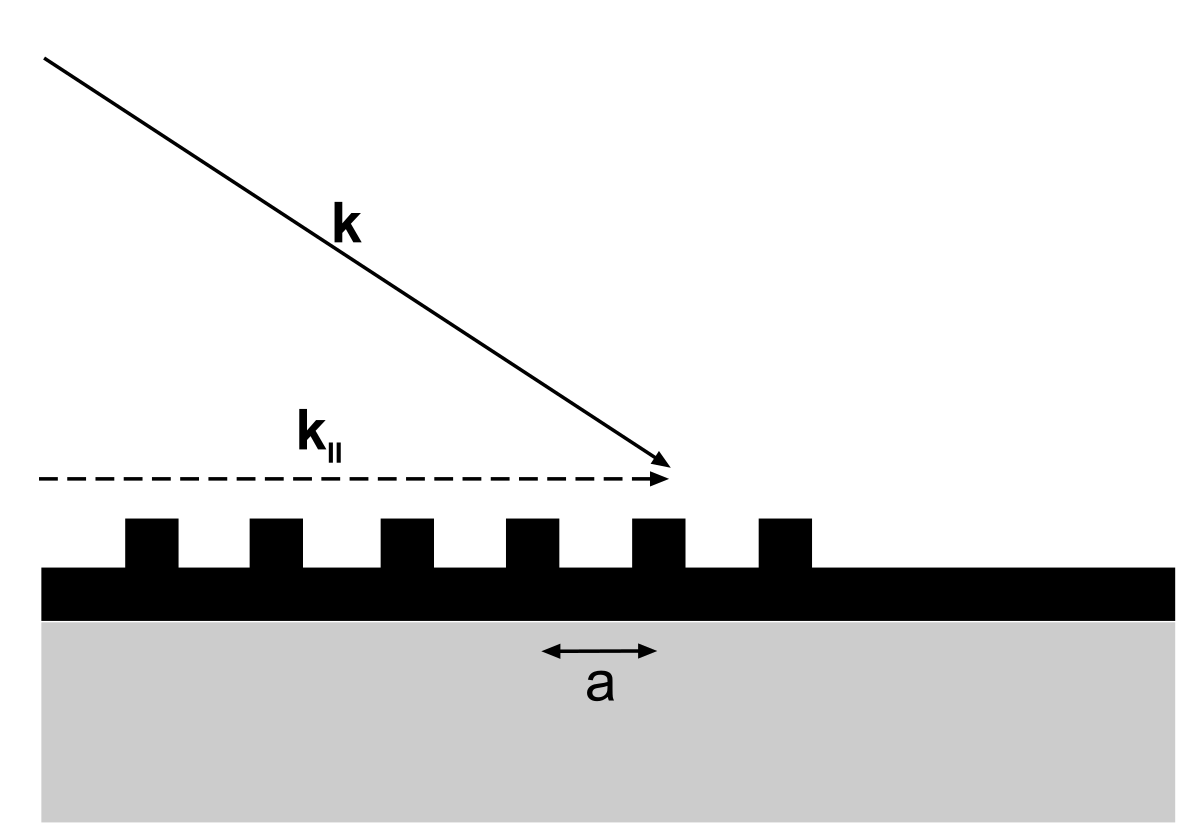
\includegraphics[width=3.5cm]{images/gitter.png}\\ \hspace{1.5cm} {[{Stefan Maier, Plasmonics}]}
            }
        \end{column}
    \end{columns}
\end{frame}

%\subsection{Große Zeemanaufspaltung}
\begin{frame}{Große Zeemanaufspaltung}
    \pause
    \begin{columns}
        \begin{column}{0.5\textwidth}
            \begin{itemize}
                \item <1-> Aufspaltung der Energieniveaus im Magnetfeld
                \item <3-> Magnetfeld in Voigt-Geometrie \rightarrow parallel zur Probenoberfläche 
                \item <4-> Aufspaltung von Leicht- (lh) und Schwerloch (hh) in jeweils 2 Niveaus
                \item <5-> blau, rot $\sigma \text{-Übergänge}$ \rightarrow beide zirkular Polarisiert in x-y-Ebene 
                \rightarrow Unterschied der Drehrichtung
                \item <6-> Schwerlochübergang am wahrscheinlichsten
                \item <7-> bei tiefen Temperaturen quasi nur Übergange in das Schwerlochband
            \end{itemize}
        \end{column}
        \begin{column}{0.5\textwidth}
            \centering
            \only <2->{
            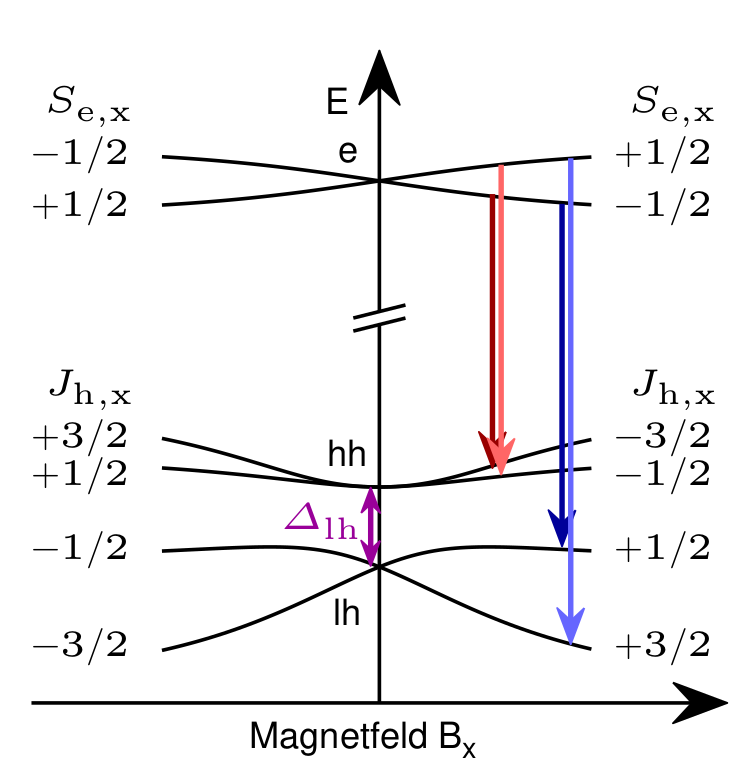
\includegraphics[scale=0.2]{images/zeeman.png}\\[-0.5\baselineskip]{[Felix Spitzer, Dissertation]}}
        \end{column}
    \end{columns}
\end{frame}

%\subsection{Magnetisch kontrollierte direktionale Lichtemission}
\begin{frame}{Magnetisch kontrollierte direktionale Lichtemission}
    \pause
    \begin{columns}
        \begin{column}{0.5\textwidth}
            \begin{itemize}
                \item <1-> Beschreibt wie mit Hilfe eines
                angelegten äußeren Magnetfelds die Lichtemission einer Probe gerichtet
                werden kann. 
                \bigskip   
                \item <3-> Laser erzeugt im Quantentopf der
                Probe Exzitonen als Quelle der Strahlung
                \bigskip   
                \item <4-> Emission der Exzitonen besitzen vorgegebene zirkulare Polarisation
                \bigskip
                \item <5->  Deckschicht: \SI{30}{\nano\meter}
                \item <5->  Quantentopf: \SI{10}{\nano\meter}
                \item <5->  Puffer: \SI{4,6}{\micro\meter}
            \end{itemize}
        \end{column}
        \begin{column}{0.5\textwidth}
            \centering
            \only <2->{
                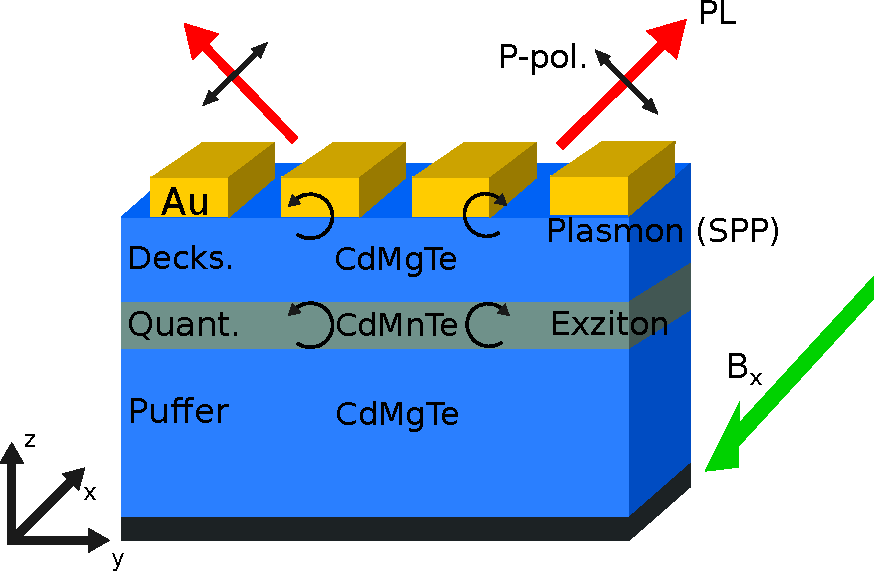
\includegraphics[scale=0.35]{images/Probe_komplett.pdf}\\[-0.5\baselineskip]
                }
        \end{column}
    \end{columns}
\end{frame}

\begin{frame}{Magnetisch kontrollierte direktionale Lichtemission}
    \begin{columns}
        \begin{column}{0.5\textwidth}
            \begin{itemize}
                \item <1-> für $B_{x} = 0$ zirkulare Emission der Exzitonen nur in der x-y-Ebene
                \item <3-> für $B_{x} \neq 0$ zirkulare Emission der Exzitonen erscheinen in der y-z-Ebene
                elliptisch polarisiert 
                \item <4-> Grad der zirkularen Polarisation
                \begin{equation*}
                    P_c \approx \frac{2}{3} \frac{\Delta_\text{h,F}(T)}{\Delta_\text{lh}} \propto B
                    \label{eq:pc}
                \end{equation*}
                \item <5-> Exzitonen können mit Plasmonen mit gleicher Polarisation koppeln 
                \item <6-> Plasmonen emittieren als Licht \rightarrow direktionale Lichtemission
                \item <7-> Steuerung durch Magnetfeld möglich \rightarrow transversale magnetische Führung der Lichtemission (TMRLE)
            \end{itemize}
        \end{column}
        \begin{column}{0.5\textwidth}
            \centering
            \only <2->{
                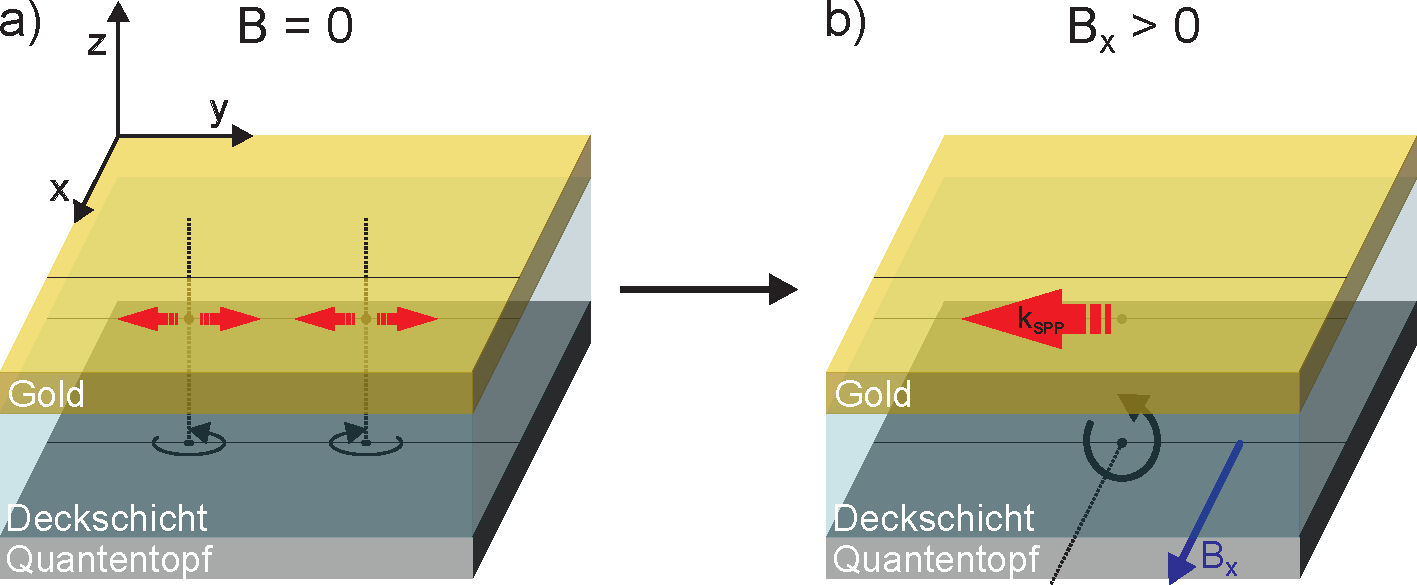
\includegraphics[scale=0.25]{images/exziton.pdf}\\[-0.5\baselineskip]{[Lars Klompmaker, Masterarbeit]}
             }
        \end{column}
    \end{columns}
\end{frame}

%\subsection{Temperaturabhängigkeit der magnetisch kontrollierten direktionale Lichtemission}
\begin{frame}{Temperaturabhängigkeit der magnetisch kontrollierte direktionale Lichtemission}
    \begin{columns}
        \begin{column}{0.5\textwidth}
            \begin{itemize}
                \item <1-> $\Delta_\text{h,F}(T)$ ist temperaturabhängig  
                \rightarrow $\Delta_\text{h,F}(T) = xN_0\beta \bigl< S^\text{Mn}_{z} \bigr>$
                \item <2-> $\bigl< S^\text{Mn}_{z} \bigr>$ ist die mittlere thermische Spinausrichtung der Mn-Ionen entlang des angelegten
                Magnetfelds 
                \item <3->
                \begin{align*}
                    \label{eq:S}
                    \bigl< S^\text{Mn}_{z} \bigr> &= S_\text{eff} B_\text{$\frac{5}{2}$} \left(\frac{5}{2}\frac{g_\text{Mn} \mu_\text{B} B }{T_\text{eff} k_\text{B}} \right)\text{.}
                \end{align*}
                \bigskip
                \item <4-> anschaulich \rightarrow mit steigender Temperatur wird die Spinausrichtung schlechter 
                \item <5-> $P_\text{c}$ sinkt \rightarrow Verlust der Direktionaltät
                %\item <->
            \end{itemize}
        \end{column}
        \begin{column}{0.5\textwidth}
            \centering
            \only <1->{
                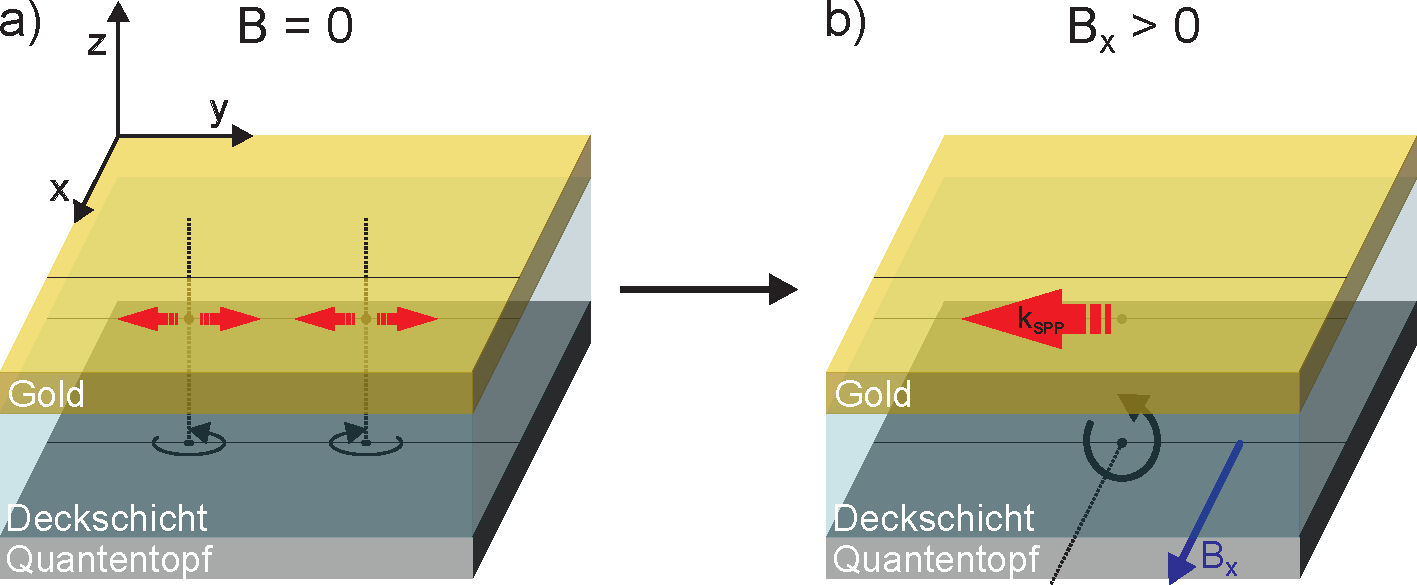
\includegraphics[scale=0.25]{images/exziton.pdf}\\[-0.5\baselineskip]{[Lars Klompmaker, Masterarbeit]}                
            }
            %\only <6->{
            %    \bigskip 
            %    \begin{align*}
            %        P_c \approx \frac{2}{3} \frac{\Delta_\text{h,F}(T)}{\Delta_\text{lh}} \propto B
            %    \end{align*}
            %}
        \end{column}
    \end{columns}
\end{frame}
%\begin{frame}{titel}
%    \pause
%    \begin{columns}
%        \begin{column}{0.5\textwidth}
%            \begin{itemize}
%                \item <->
%                \item <->
%                \item <->
%                \item <->
%                \item <->
%                \item <->
%            \end{itemize}
%        \end{column}
%        \begin{column}{0.5\textwidth}
%            \centering
%            \only <->{
%                \includegraphics[scale=0.25]{images/}\\[-0.5\baselineskip]
%                \hspace{1.5cm}}%\href{www. ...}{[name, paper]}
%             }
%        \end{column}
%    \end{columns}
%\end{frame}


\section{Experimenteller Aufbau und Durchführung}
%\subsection{Experimenteller Aufbau}
%\begin{frame}{Experimenteller Aufbau}
%    \pause
%    \begin{columns}
%        \begin{column}{0.5\textwidth}
%            \begin{itemize}
%                \item <1-> Hauptbestandteile
%                \begin{itemize}
%                    \item <2-> Festkörperlaser (grün) $\lambda= \SI{552}{\nano\meter}$ 
%                    \item <3-> Probe 
%                    \item <4-> Spektrometer  
%                \end{itemize}
%                \item <5-> ebenfalls Bestandteile sind
%                \begin{itemize}
%                    \item <4-> Durchfluss-Kryostat, Spulenpaar ($B = \SI{0,5}{\tesla}$)
%                    \item <5-> Tief- und Langpass
%                    \item <6-> BSC, Mikroskop Objektiv, Spiegel, Linsen
%                    \item <7-> Glan Thompson Prisma, Kamera, $\lambda /2$-Plättchen
%                \end{itemize}
%            \end{itemize}                
%        \end{column}
%        \begin{column}{0.5\textwidth}
%            \centering
%            \only <2->{
%            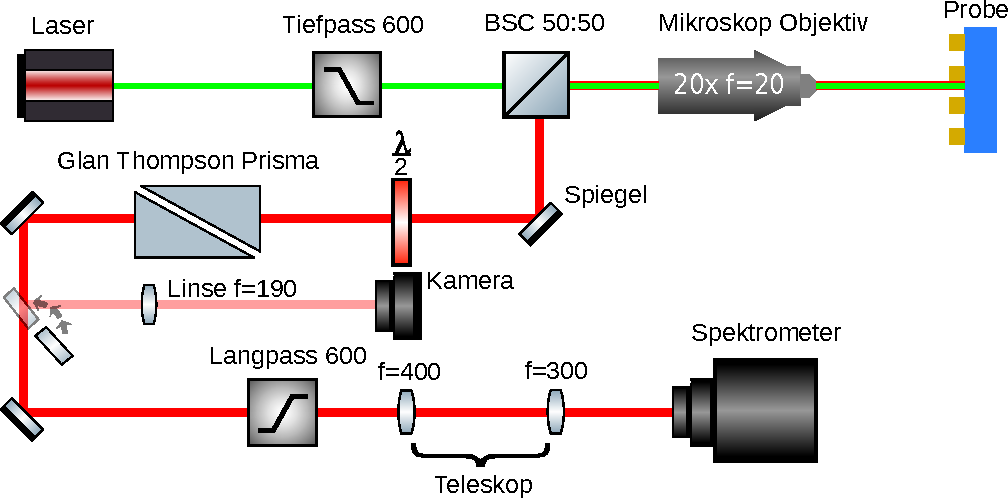
\includegraphics[scale=0.45]{images/setup.pdf}\\[-0.5\baselineskip]
%            }
%        \end{column}
%    \end{columns}
%\end{frame}


\begin{frame}{Experimenteller Aufbau}
    \pause
    \centering
    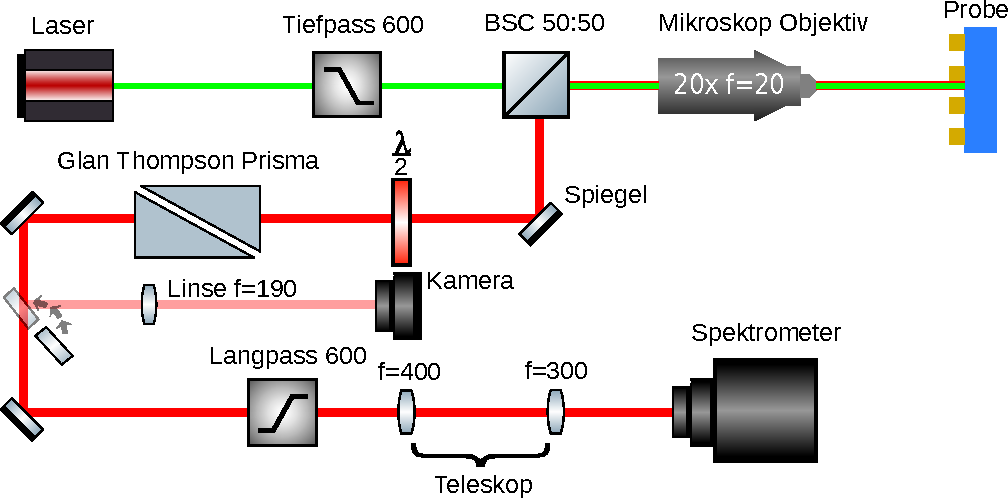
\includegraphics[scale=0.6]{images/setup.pdf}\\[-0.5\baselineskip]
\end{frame}


%\subsection{Experimentelle Durchführung}
\begin{frame}{Experimentelle Durchführung}
    \pause
    \begin{columns}
        \begin{column}{0.5\textwidth}
            \begin{itemize}
                \item <1-> Probe in den Fokus Mikroskopobjektivs 
                \bigskip
                \item <3-> Temperatureinstellung 
                    %\begin{itemize}
                    %    \item <4-> durch Heliumfluss und Heizelement
                    %\end{itemize}
                \bigskip
                \item <4-> Messung des Hintergrunds
                \bigskip
                \item <5-> abwechselndes aufnehmen von Spektren bei pos. und neg. Magnetfeld
                    %\begin{itemize}
                    %    \item <6-> 16 Einzelbildern mit jeweils 3 Sekunden Belichtungszeit, die aufaddiert werden
                    %    (Einzelbilder da sonst Sättigung der CCD)
                    %    \item <7->  insg. 26 Spektren bei pos. und neg. Magnetfeld
                    %    (Wechsel wirkt Störeffekten entgegen z.B. Änderungen der Laserintensität über Zeitraum)
                    %\end{itemize}
                \bigskip
                \item <6-> Nach Messung wird nächste Temperatur eingestellt
            \end{itemize}                
        \end{column}
        \begin{column}{0.5\textwidth}
            \centering
            %\only <2->{
            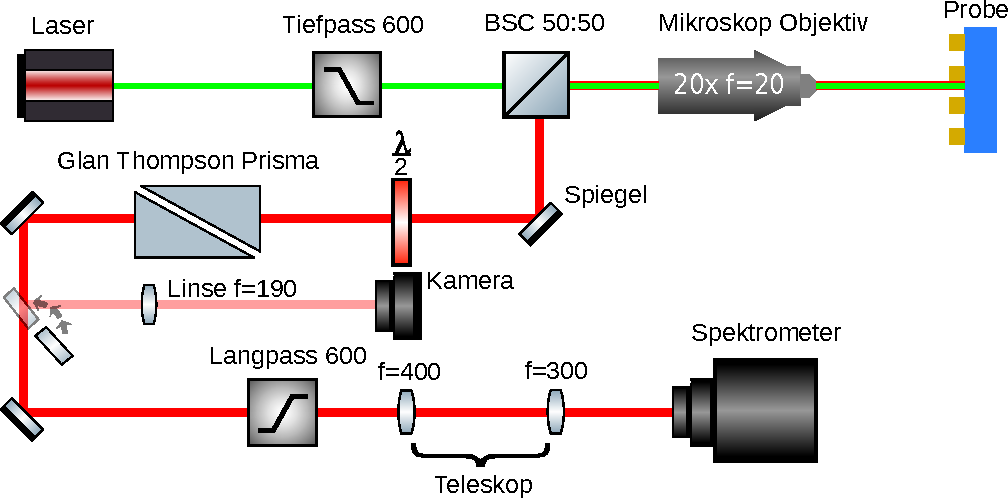
\includegraphics[scale=0.45]{images/setup.pdf}\\[-0.5\baselineskip]
            %}
        \end{column}
    \end{columns}
\end{frame}
%%\begin{frame}{titel}
%    \pause
%    \begin{columns}
%        \begin{column}{0.5\textwidth}
%            \begin{itemize}
%                \item <->
%                \item <->
%                \item <->
%                \item <->
%                \item <->
%                \item <->
%            \end{itemize}
%        \end{column}
%        \begin{column}{0.5\textwidth}
%            \centering
%            \only <->{
%                \includegraphics[scale=0.25]{images/}\\[-0.5\baselineskip]
%                \hspace{1.5cm}}%\href{www. ...}{[name, paper]}
%             }
%        \end{column}
%    \end{columns}
%\end{frame}
\section{Beschreibung des Probenkörpers}
\begin{frame}{Beschreibung des Probenkörpers}
    \pause
    \begin{columns}
        \begin{column}{0.5\textwidth}
            \begin{itemize}
                \item <1-> 3 Schichten plus Gitter
                \begin{itemize}
                    \item <2-> Substrat: GaAs (hier schwarz)
                    \bigskip
                    \item <3-> Pufferschicht: CdMgTe $\SI{4,6}{\micro\meter}$
                    \item <3-> Quantentopf: CdMnTe $\SI{10}{\nano\meter}$
                    \item <3-> Deckschicht: CdMgTe $\SI{30}{\nano\meter}$ 
                    \bigskip
                    \item <4-> Goldgitter mit einer Periode von $\SI{250}{\nano\meter}$
                \end{itemize}
                \bigskip
                \item <5-> CdMnTe ist ein semimagnetischen Halbleiter (DMS)
                \item <6-> Im QW entstehen Exzitonen
                \item <7-> zwischen Deckschicht und Goldgitter entstehen Plasmonen
            \end{itemize}
        \end{column}
        \begin{column}{0.5\textwidth}
            \centering        
            \only <1->{    
            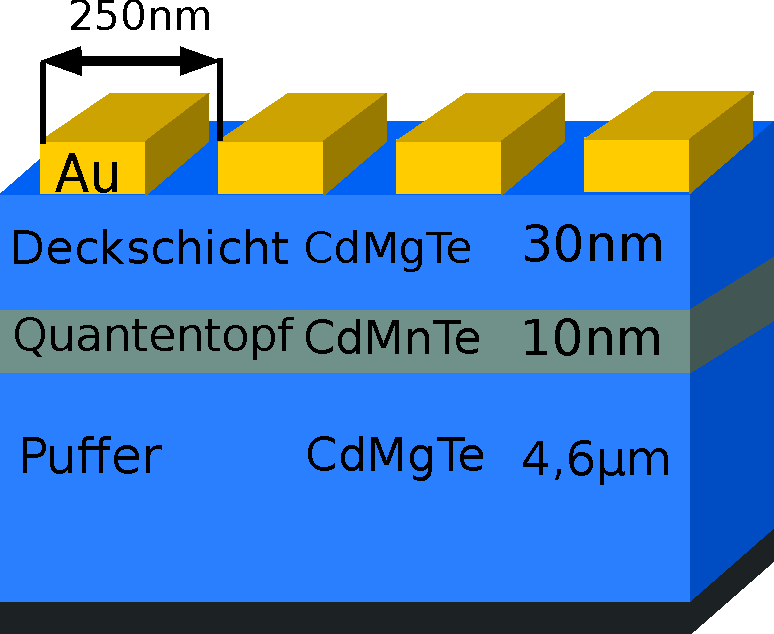
\includegraphics[scale=0.3]{images/probe.pdf}\\[-0.5\baselineskip]  }              
        \end{column}
    \end{columns}
\end{frame}
%\begin{frame}{titel}
%    \pause
%    \begin{columns}
%        \begin{column}{0.5\textwidth}
%            \begin{itemize}
%                \item <->
%                \item <->
%                \item <->
%                \item <->
%                \item <->
%                \item <->
%            \end{itemize}
%        \end{column}
%        \begin{column}{0.5\textwidth}
%            \centering
%            \only <->{
%                \includegraphics[scale=0.25]{images/}\\[-0.5\baselineskip]
%                \hspace{1.5cm}}%\href{www. ...}{[name, paper]}
%             }
%        \end{column}
%    \end{columns}
%\end{frame}
\section{Auswertung der Messdaten und Diskussion}
%\subsection{Photolumineszenz und Direktionalität bei konstanter Temperatur}

\begin{frame}{Photolumineszenz bei \SI{4}{\kelvin}}
    \pause
    \begin{columns}
        \begin{column}{0.5\textwidth}
            \begin{itemize}
                \item <1-> Messung der Photolumineszenz bei $\SI{4}{\kelvin}$ 
                \centering
                \only <2-> {
                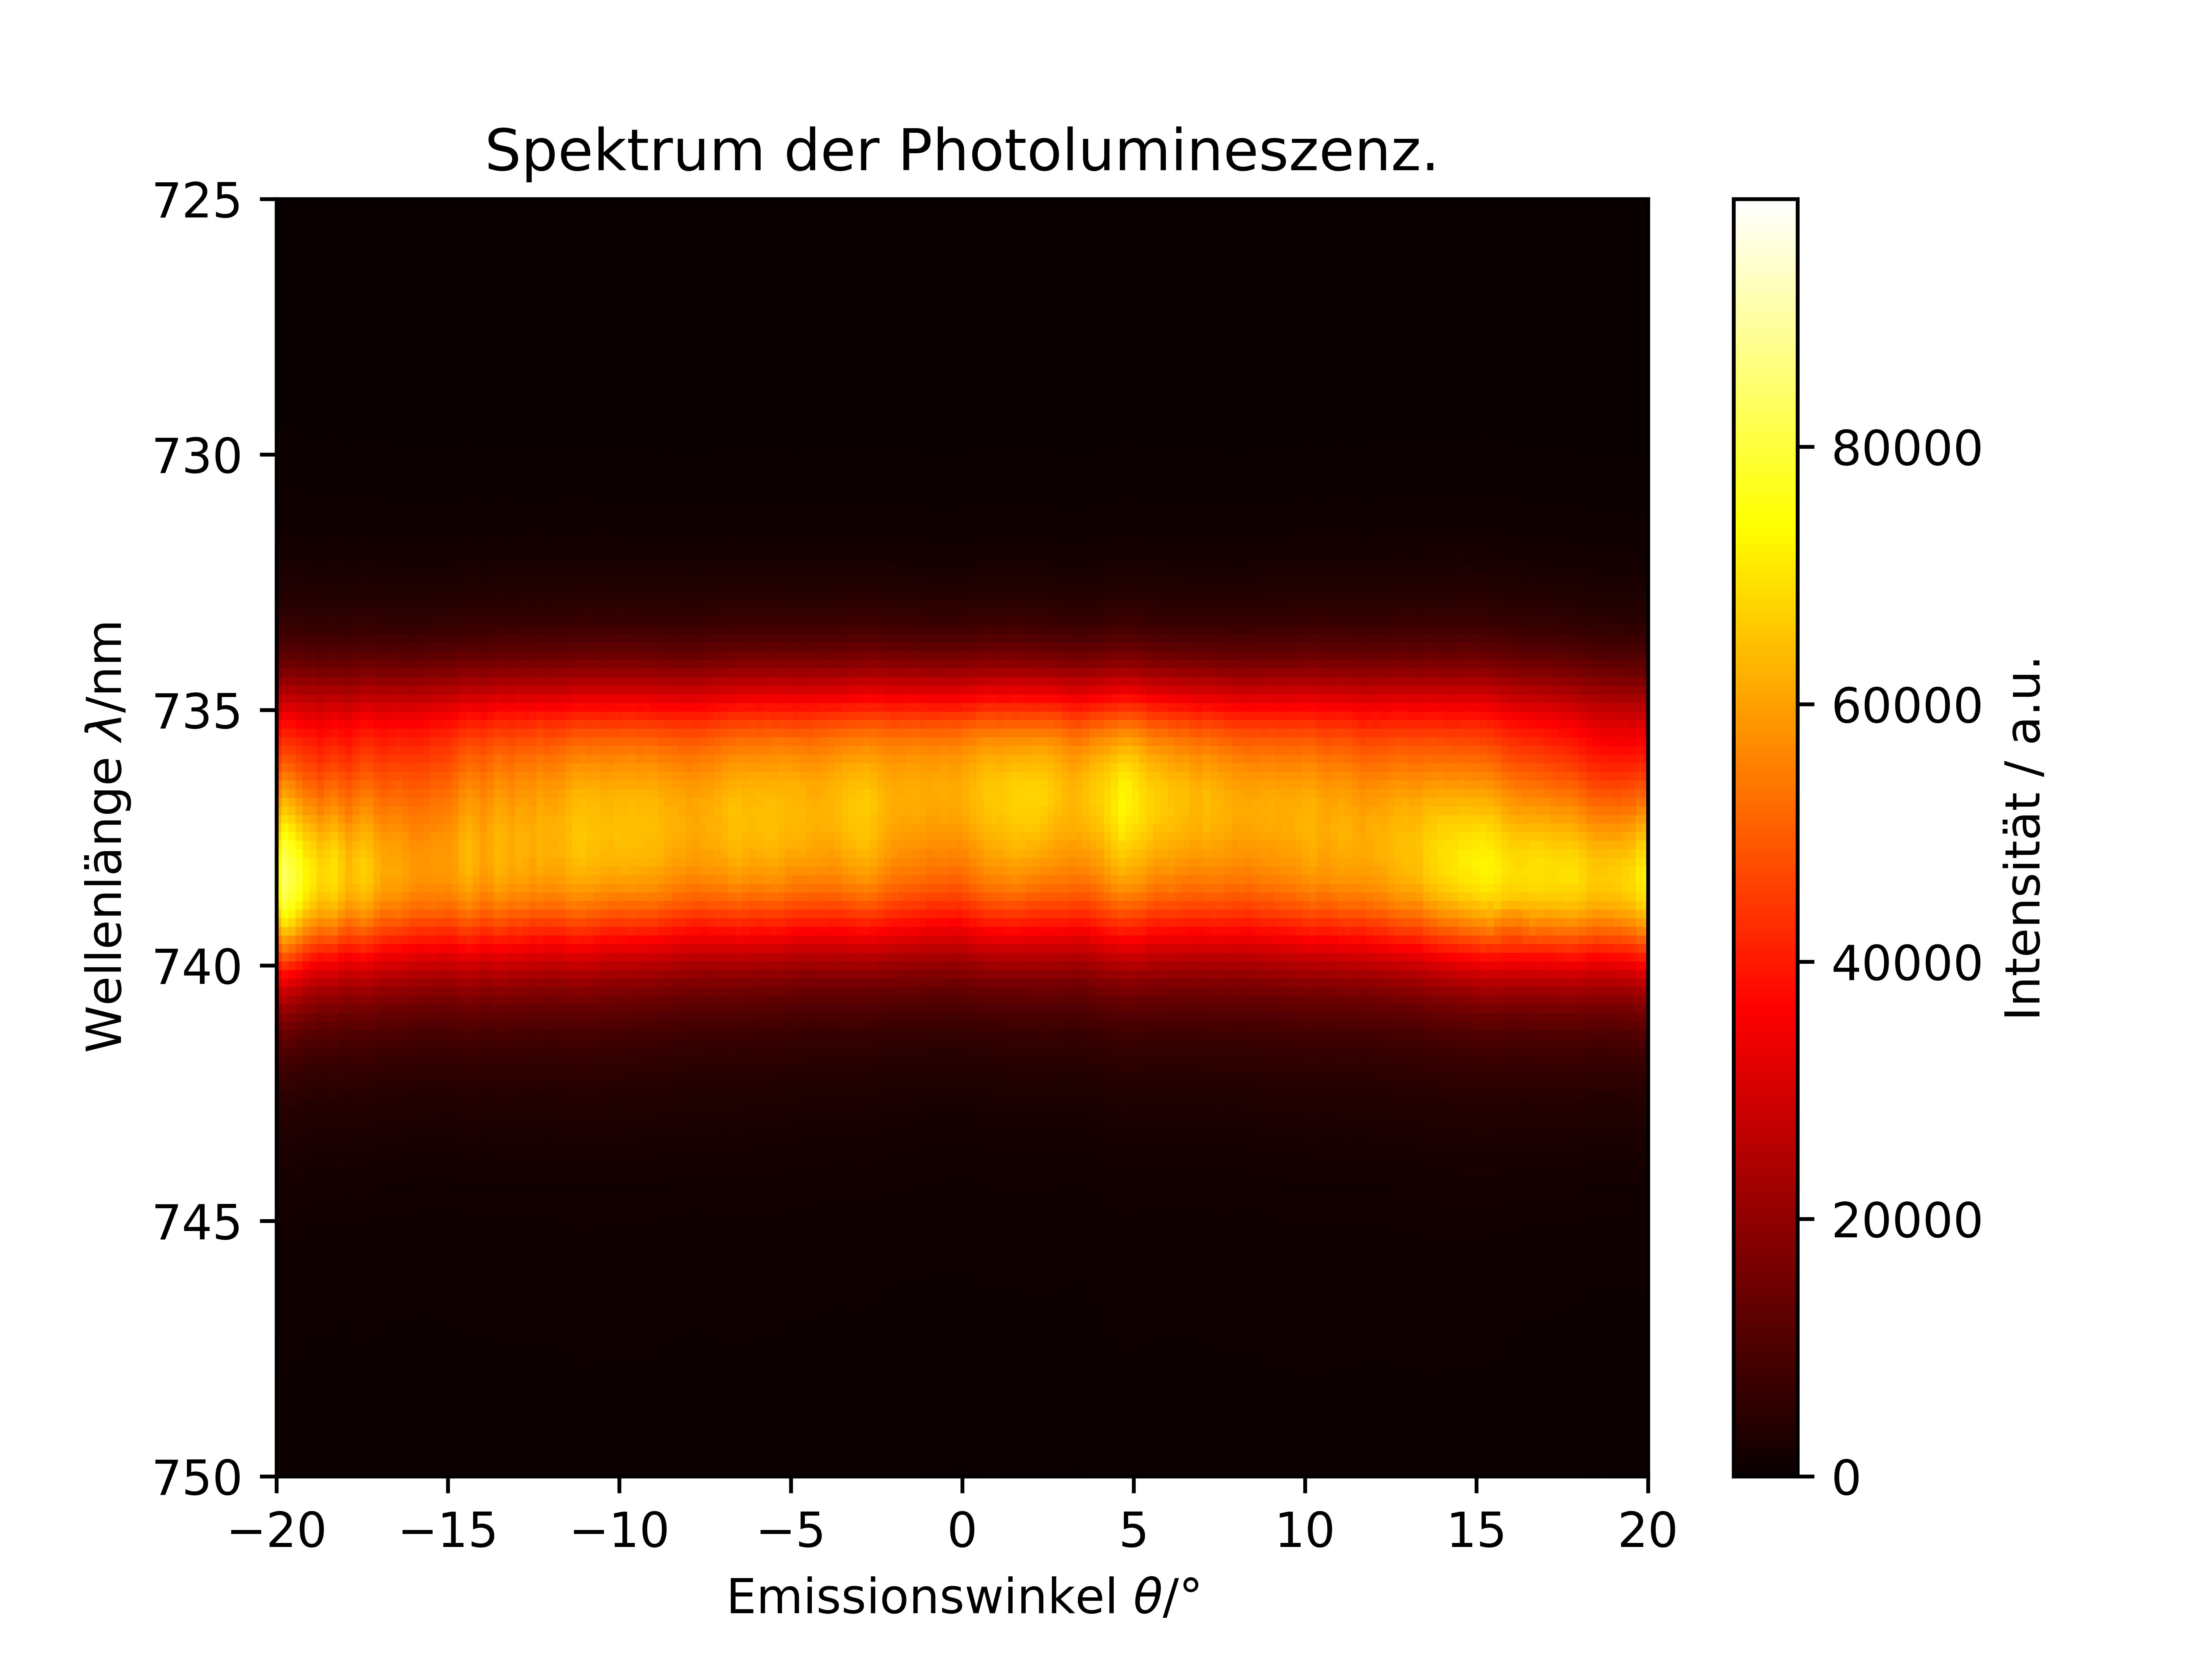
\includegraphics[scale=0.4]{images/colormap__intensity_photolumineszenz_022818A 250nm 4K 2020-07-14.png}\\[-0.5\baselineskip]                
                }
            \end{itemize}
        \end{column}
        \begin{column}{0.5\textwidth}
            \begin{itemize}
                \item <3-> Maximum der Emission bei $\SI{737}{\nano\meter}$ 
                \centering
                \only <3-> {
                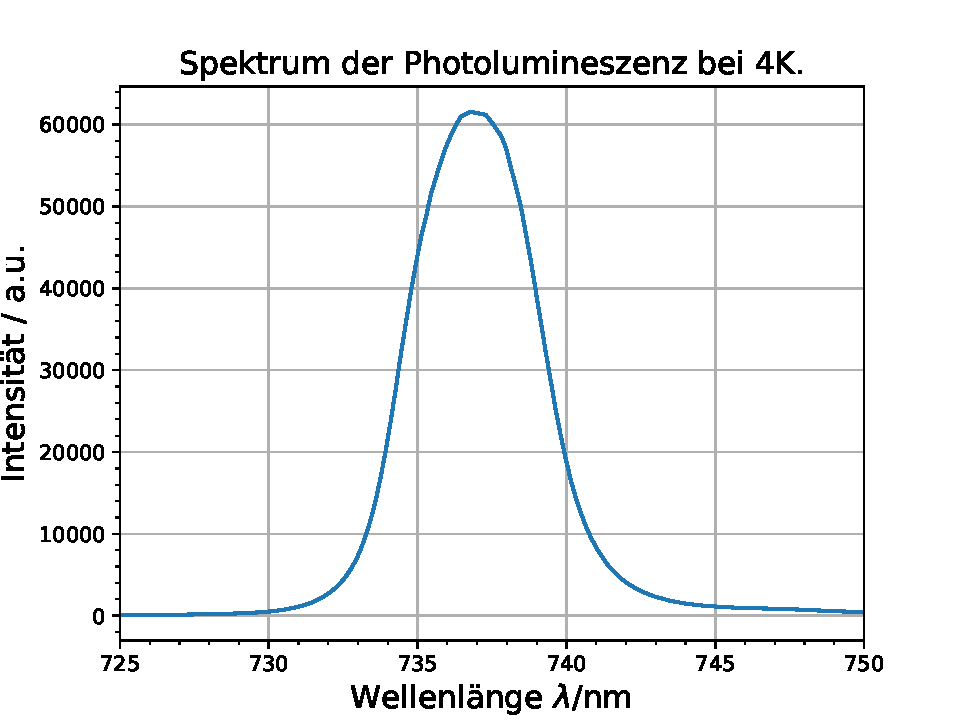
\includegraphics[scale=0.4]{images/max_value_Pl_single.pdf}\\[-0.5\baselineskip]       
                }
            \end{itemize}
        \end{column}
    \end{columns}
\end{frame}

%\begin{frame}{Relative Änderung bei \SI{4}{\kelvin}}
%    \begin{itemize}
%        \item <1-> Richtungsabhängigkeit der Lichtemission
%        \centering
%        \only <1-> {
%        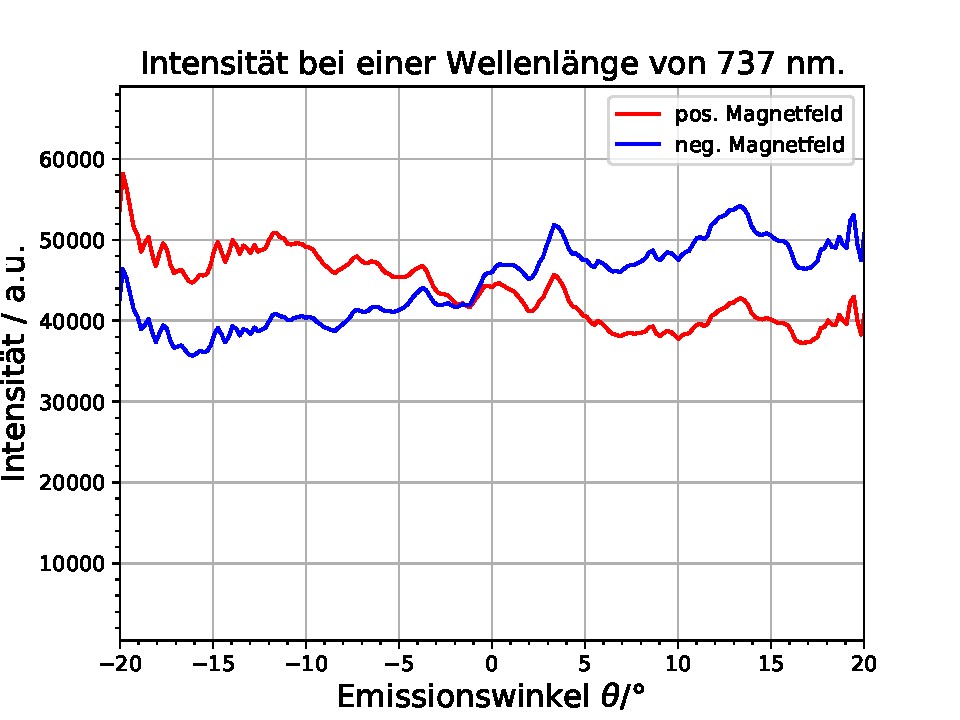
\includegraphics[scale=0.4]{images/positive_and_negative_intensity_at_specific_wavelength_737_nm_022818A 250nm 4K 2020-07-14.pdf}\\[-0.5\baselineskip]                
%        }
%    \end{itemize}
%\end{frame}

\begin{frame}{Relative Änderung bei \SI{4}{\kelvin}}
    \begin{columns}
        \pause
        \begin{column}{0.5\textwidth}
            \begin{itemize}
                \item <2-> Richtungsabhängigkeit der Lichtemission
                \item <3-> Quantifizierung der relativen Änderung der Intensität
                \begin{equation*}
                    \rho = \frac{I_\text{B+} - I_\text{B-} }{ I_\text{B+} + I_\text{B-} }.
                \end{equation*}
                $\rho$ gibt die Änderung der Intensität bei Umpolung des Magnetfelds an.
                \item <6-> Bspl. positive Emissionswinkel \rightarrow relative Änderung $\rho$ negativ 
                \rightarrow mehr Licht bei negativem Magnetfeld emittiert als bei positivem Magnetfeld
                \item <7-> beste Steuerung im Bereich von $\SI{738}{\nano\meter}$ bis $\SI{740}{\nano\meter}$\\
                und $\theta = \pm \SI{11}{\degree}$ bis $\theta = \pm \SI{13,5}{\degree}$
            \end{itemize}
        \end{column}
        \begin{column}{0.5\textwidth}
            \centering 
            \only <1-3> {%
            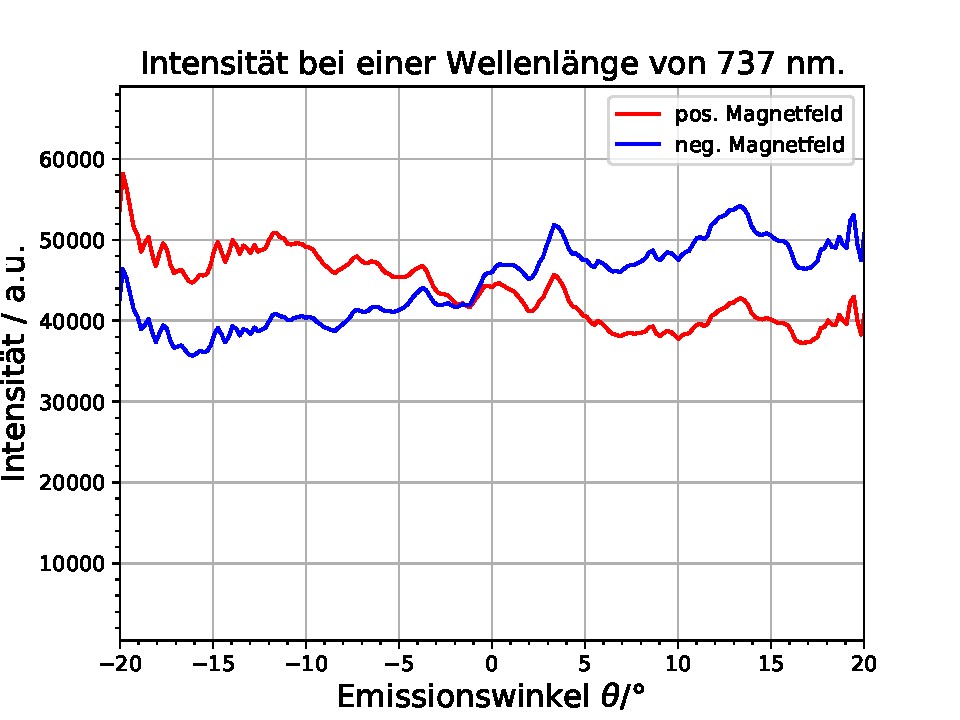
\includegraphics[scale=0.4]{images/positive_and_negative_intensity_at_specific_wavelength_737_nm_022818A 250nm 4K 2020-07-14.pdf}\\[-0.5\baselineskip]%
            }%
            \only <4> {%
            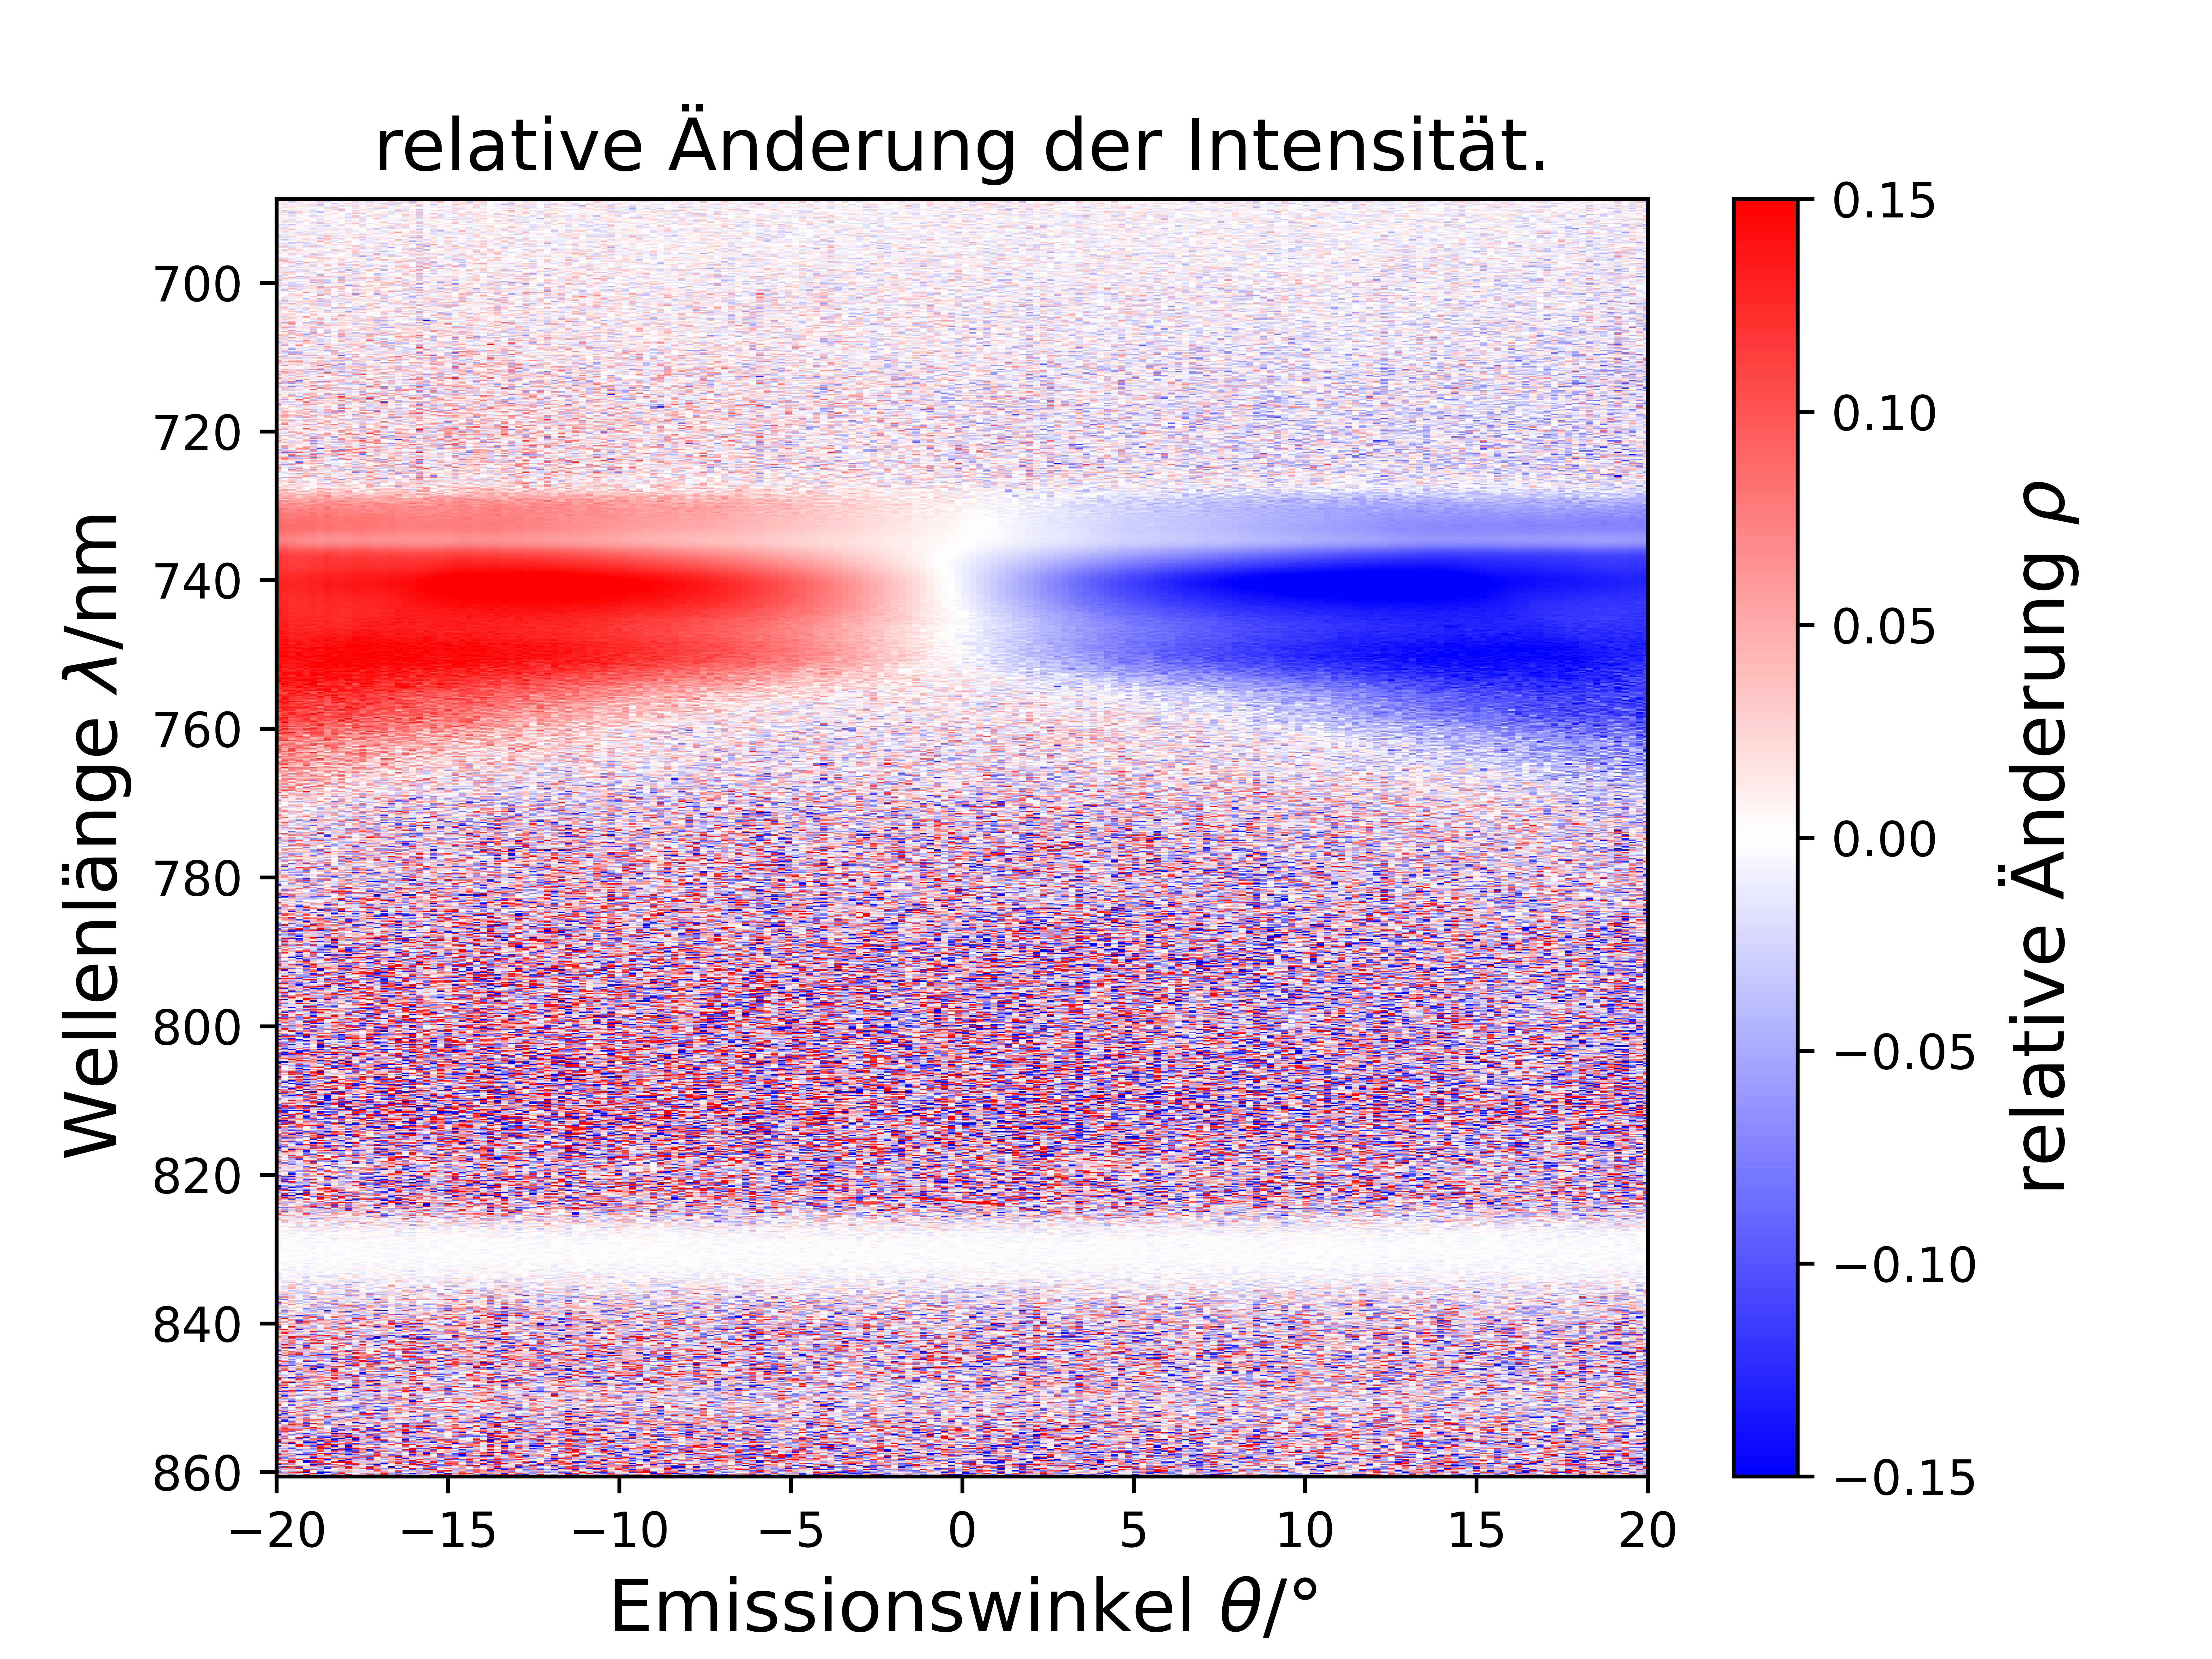
\includegraphics[scale=0.4]{images/colormap_rel_change_intensity_022818A 250nm 4K 2020-07-14_komplett.png}\\[-0.5\baselineskip]%
            }%
            \only <5-> {%
            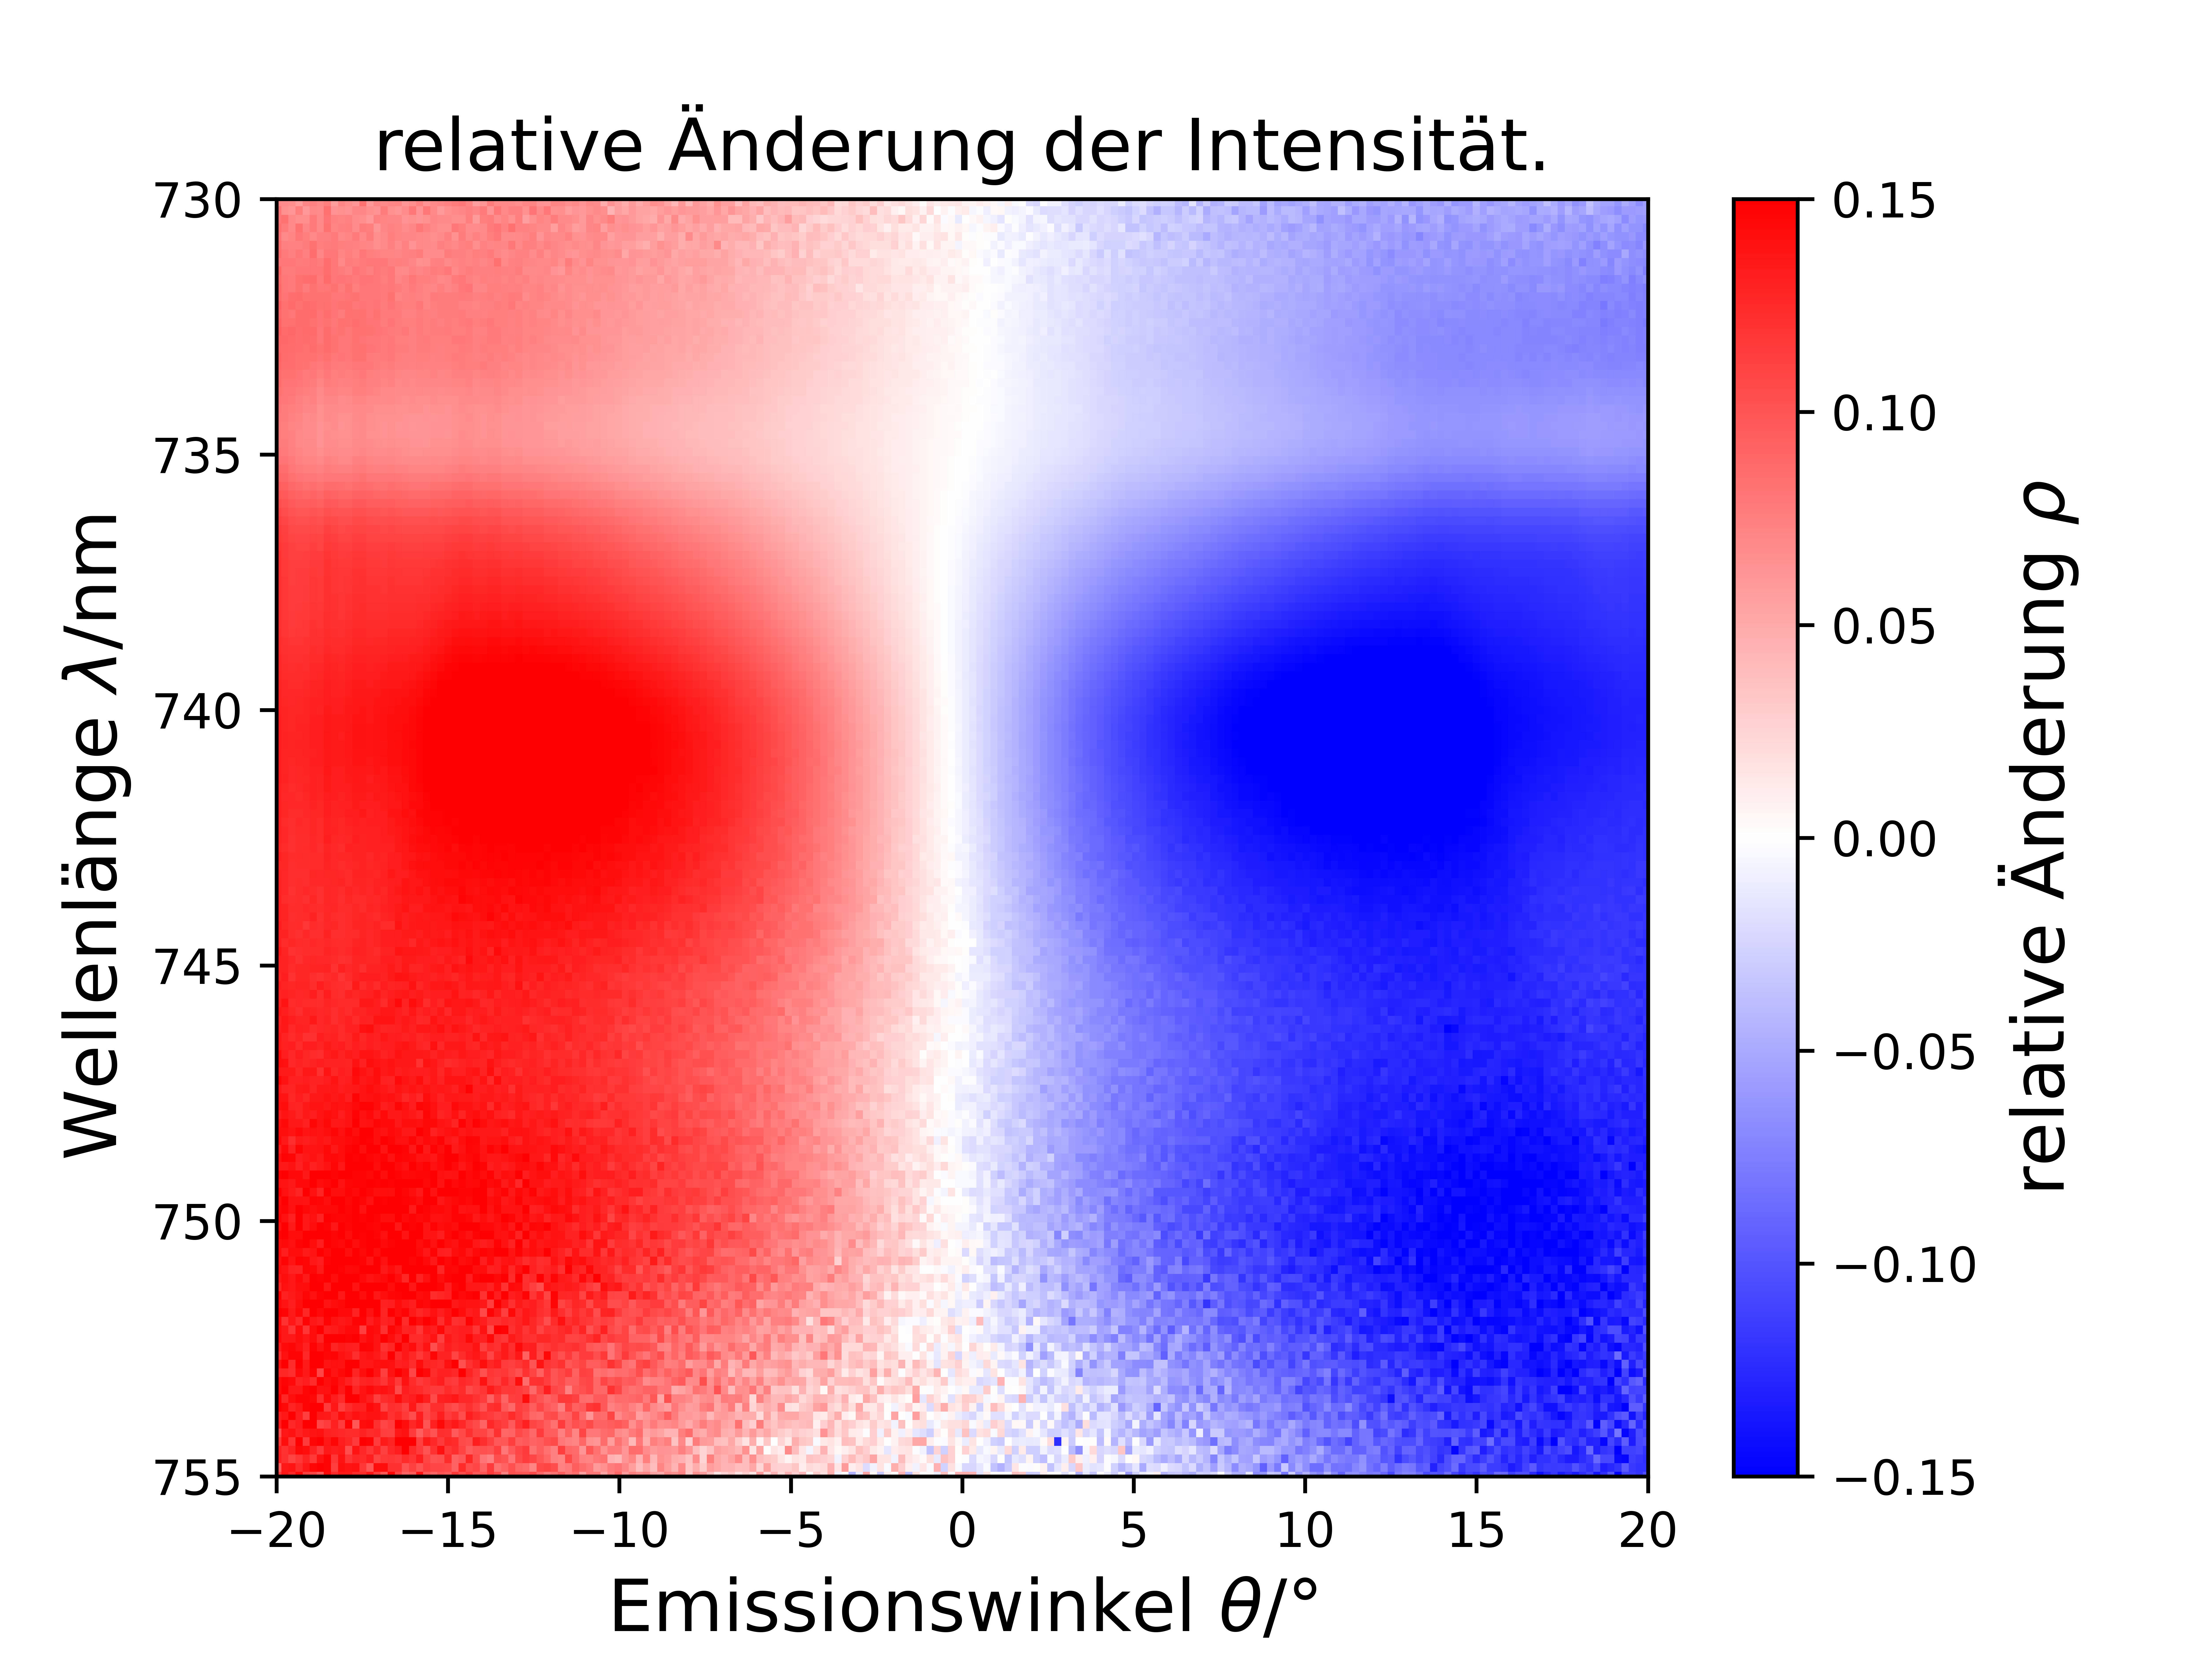
\includegraphics[scale=0.4]{images/colormap_rel_change_intensity_022818A 250nm 4K 2020-07-14.png}\\[-0.5\baselineskip]%           
            }%
        \end{column}
    \end{columns}
\end{frame}


\begin{frame}{Relative Änderung bei \SI{4}{\kelvin}}
    %\pause
    \begin{columns}
        \begin{column}{0.5\textwidth}
            \begin{itemize}
                \item <1-> relative Änderung $\rho$ in Abhängigkeit von Emissionswinkel $\theta$
                \item <2-> antisymmetrisch bis auf eine kleine Abweichung am Nullpunkt 
                \item <3-> Antisymmetrie von Theorie vorhergesagt und bestätigt
                \bigskip
                \item <4-> Definition: Direktionalität
                \begin{equation*}
                    C= \frac{\rho(-\theta)-\rho(\theta)}{2}                    
                \end{equation*}
                \item <6-> steigende Verbesserung der Steuerbarkeit der Lichtemission bis $\theta = \pm \SI{13,5}{\degree}$
            \end{itemize}
        \end{column}
        \begin{column}{0.5\textwidth}
            \centering 
            \only <1-4> {%
            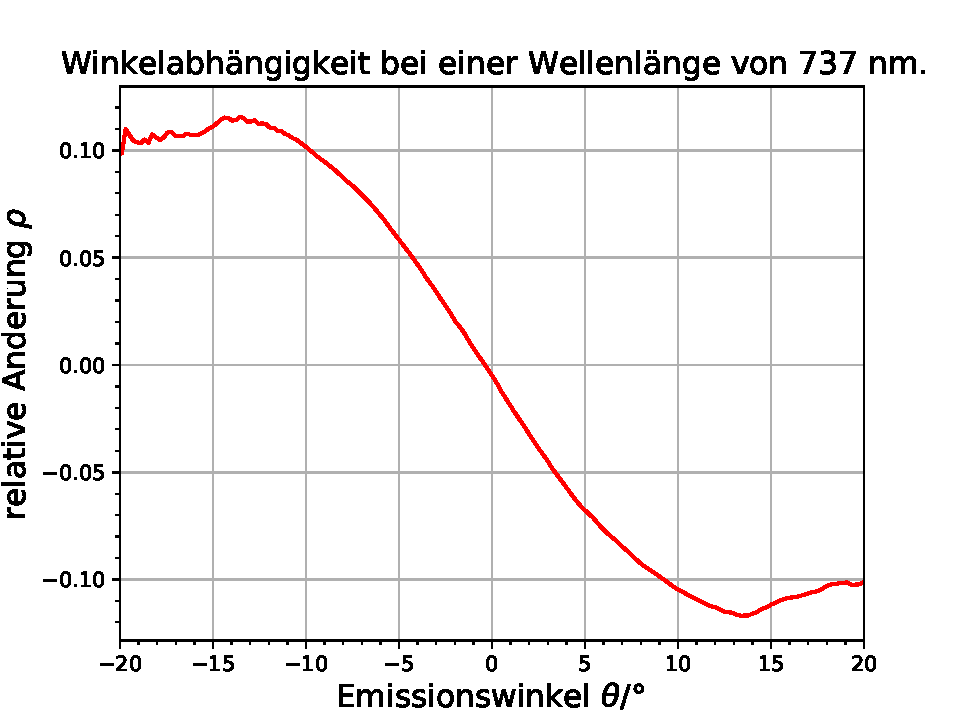
\includegraphics[scale=0.4]{images/rho_at_specific_wavelength_737_nm_022818A 250nm 4K 2020-07-14.pdf}\\[-0.5\baselineskip]%
            }%
            \only <5-> {%
            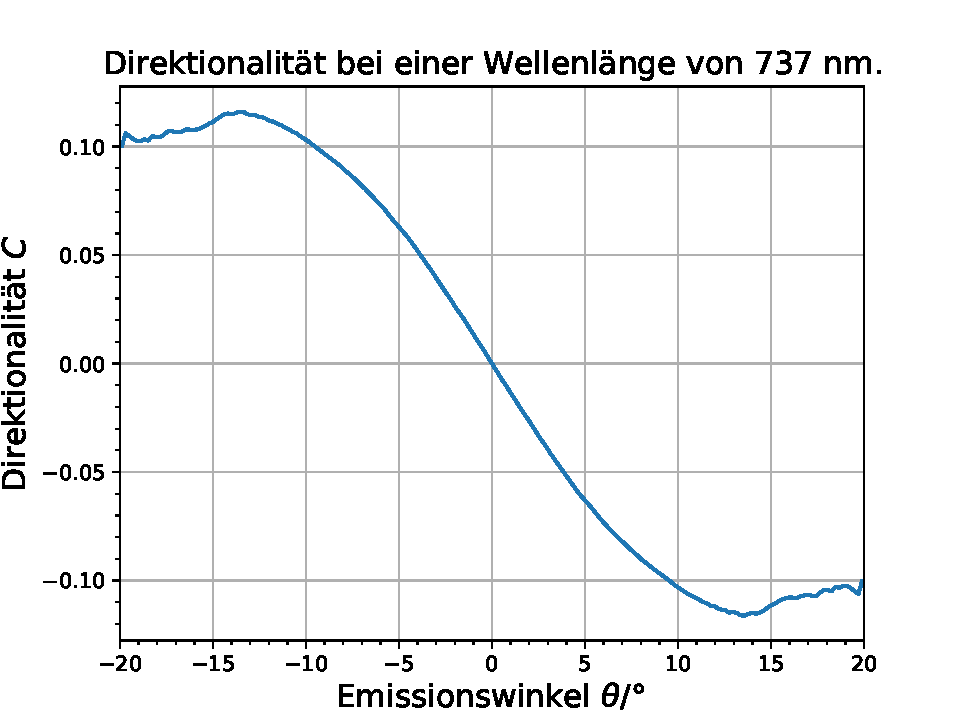
\includegraphics[scale=0.4]{images/rho_at_specific_wavelength_737_nm_022818A 250nm 4K 2020-07-14_korrigiert.pdf}\\[-0.5\baselineskip]%           
            }%
        \end{column}
    \end{columns}
\end{frame}

%\subsection{Temperaturabhängigkeit der Direktionalität}
\begin{frame}{Temperaturabhängigkeit der Direktionalität}
    %\pause^
    \begin{columns}
        \begin{column}{0.5\textwidth}
            \begin{itemize}
                \item <1-> Temperaturbereich $T = \SI{4}{\kelvin}\text{ bis }T = \SI{45}{\kelvin}$
                \bigskip
                \item <2-> Grad der zirkularen Polarisation sinkt mit steigender Temperatur
                \begin{align*}
                    P_c \approx \frac{2}{3} \frac{\Delta_\text{h,F}(T)}{\Delta_\text{lh}} \propto B
                \end{align*}
                \rightarrow Direktionalität sinkt                
                \rightarrow Bestätigung der vorrangestellten Theorie
            \end{itemize}
        \end{column}
        \begin{column}{0.5\textwidth}
            \centering 
            \only <1-> {%
            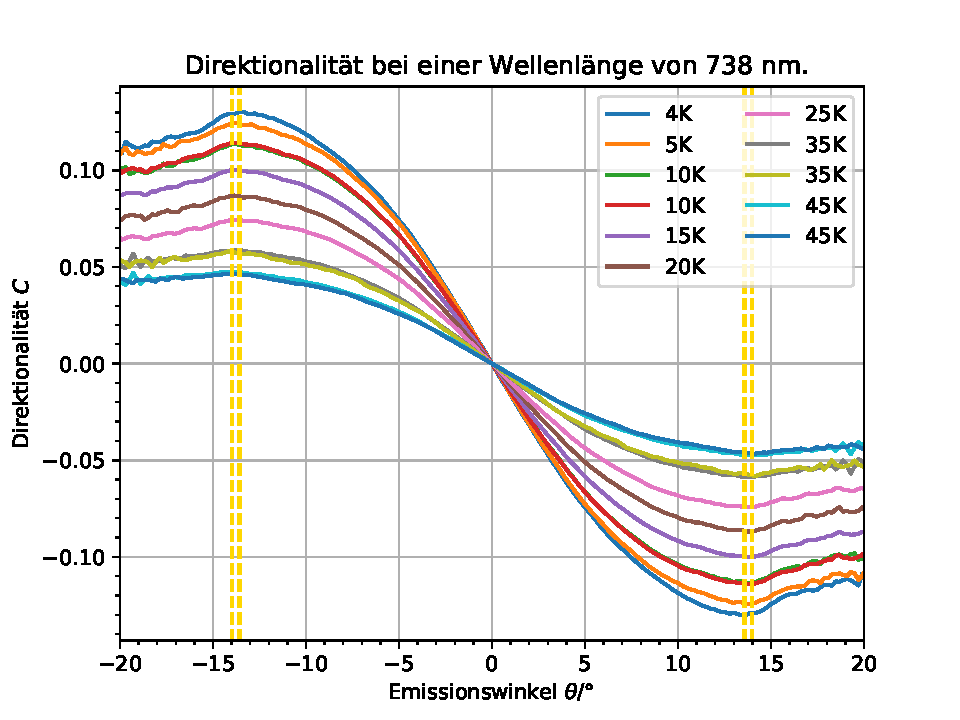
\includegraphics[scale=0.4]{images/Temperaturabhaengigkeit_rho_at_738_nm_4K5K10K10K15K20K25K35K35K45K45K_korrigiert.pdf}\\[-0.5\baselineskip]%
            }%
        \end{column}
    \end{columns}
\end{frame}

\begin{frame}{Temperaturabhängigkeit der Direktionalität}
    %\pause
    \begin{columns}
        \begin{column}{0.5\textwidth}
            \begin{itemize}       
                \item <1-> Fitfunktion
                \begin{align*}
                    C(T)&= C_0 B_\text{$\frac{5}{2}$} \left( \frac{5}{2}\frac{g_\text{Mn} \mu_\text{B} B }{T^*_\text{eff} k_\text{B}}\right)\text{,} \\
                    T^*_\text{eff} &= T + T_0 + T_\text{off}
                \end{align*}
                \item <2->  
                %\begin{align*}
                    $T: \text{gemessene/eingestellte Temperatur}$
                    $T_0:  \text{Offset durch Mangan-Paare }$
                    $T_\text{off}: \text{Offset durch äußere Einflüsse}$
                %\end{align*}
                \item <3-> Fitparameter
                \begin{align*}
                    C_0 & = \si{4,5 \pm 0,3} \\
                    T_\text{off} & = \SI{ 20 \pm 2}{\kelvin}
                \end{align*}
            \end{itemize}
        \end{column}
        \begin{column}{0.5\textwidth}
            \centering 
            \only <1-> {%
            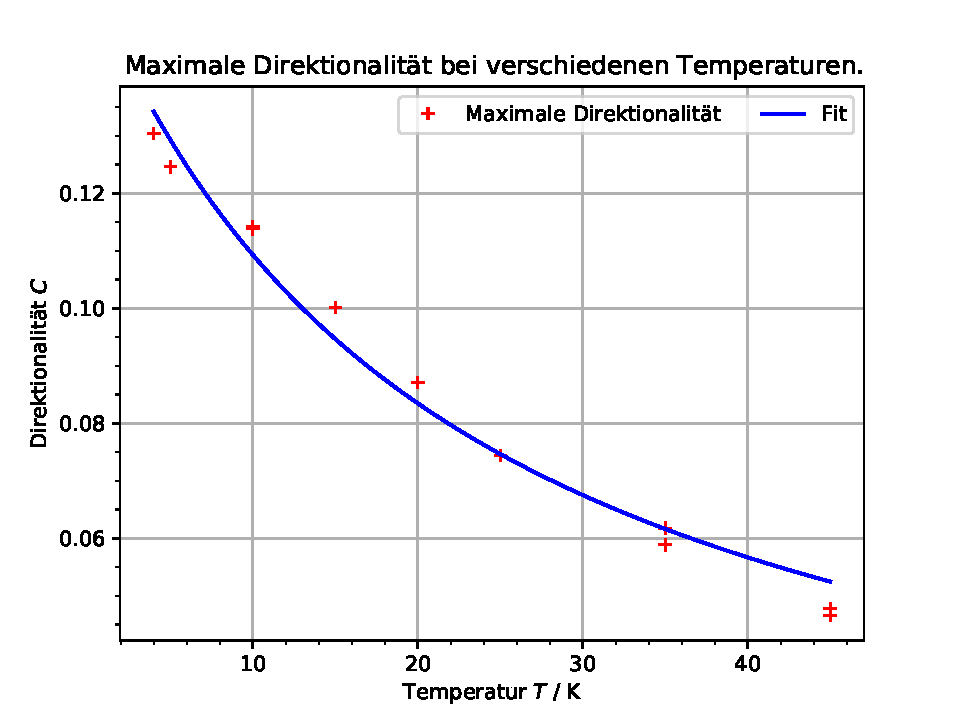
\includegraphics[scale=0.4]{images/Maximale_Rho_bei_Temperaturabhänigkeit.pdf}\\[-0.5\baselineskip]%
            }%
        \end{column}
    \end{columns}
\end{frame}

\begin{frame}{Temperaturabhängigkeit der Direktionalität}
    \begin{columns}
        \begin{column}{0.5\textwidth}
            \begin{itemize} 
                %\item Fitparameter             
                %\begin{align*} 
                %    C_0 & = \si{4,5 \pm 0,3} \\
                %    T_\text{off} & = \SI{ 20 \pm 2}{\kelvin}
                %\end{align*}
                \item <1-> Temperatur Offset $T_\text{off}  = \SI{ 20 \pm 2}{\kelvin}$ relativ groß
                \bigskip
                \item <2-> mögliche Ursache?\\ Leistungsdichte Laser $\SI{400}{\watt\per\centi\meter^2}$
                \rightarrow lokale Temperaturerhöhungen,\\ Temperatursensor nicht auf Probenoberfläche 
                \item <3-> Experiment also schlecht? 
                \bigskip
                \item <4-> Nein! \rightarrow klarer Zusammenhang zwischen Temperatur und Direktionalität
                \bigskip
                \item <5-> Temperaturabhängigkeit kann mit Gleichung gut approximiert werden \rightarrow 
                Verlauf der Direktionalität erkennbar 
            \end{itemize}
        \end{column}
        \begin{column}{0.5\textwidth}
            \centering
            \only <1-> {%
            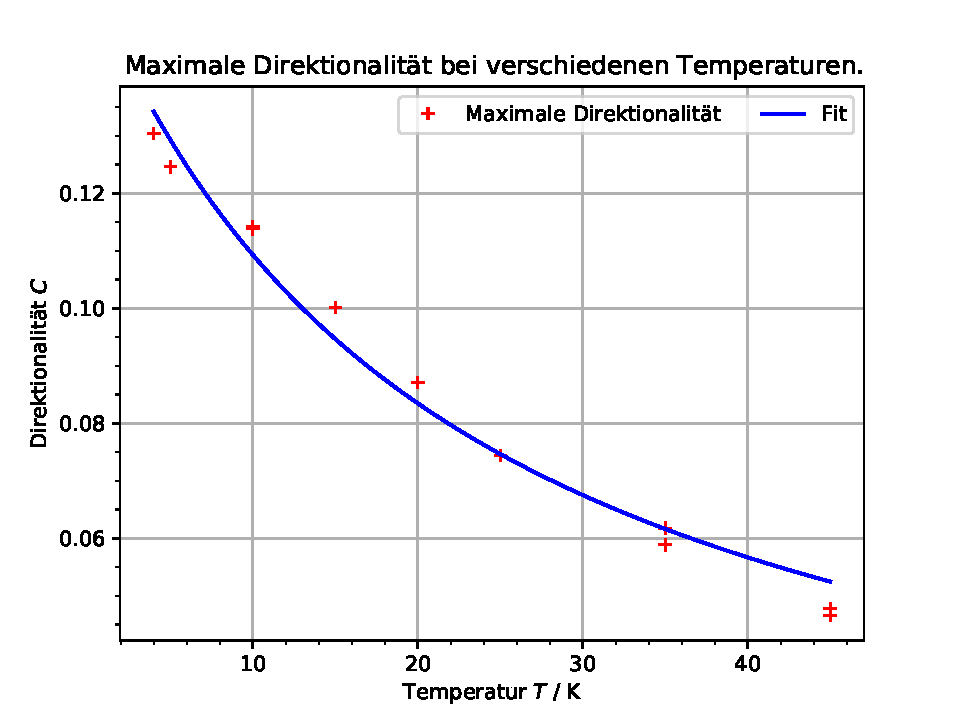
\includegraphics[scale=0.4]{images/Maximale_Rho_bei_Temperaturabhänigkeit.pdf}\\[-0.5\baselineskip]% 
            }%
        \end{column}
    \end{columns}
\end{frame}

\begin{frame}{Verbesserungen und Ausblick}
    \begin{columns}
        \begin{column}{0.5\textwidth}
            \begin{itemize}                 
                \item <1-> Verbesserungen?
                %\bigskip
                \item <2-> Messwerte pendeln um Fit 
                %\bigskip
                \begin{itemize}
                    \item <3-> \rightarrow bessere Approximation möglich
                    \item <4-> weitere Temperaturmessungen 
                \end{itemize}
                \bigskip
                \item <5-> Abhängigkeit der Leistungsdichte des Lasers
                %\bigskip
                \item <6-> Position Temperatursensor
                %\bigskip
                \item <7-> Rolle der Gitterperiode %\vspace{0.3cm}%\\~\\
                %\bigskip
                \item <8-> Zeemanaufspaltung unabhängig der Temperatur, InGaAs/InAlAs? 
            \end{itemize}
        \end{column}
        \begin{column}{0.5\textwidth}
            \centering
            \only <1-> {%
            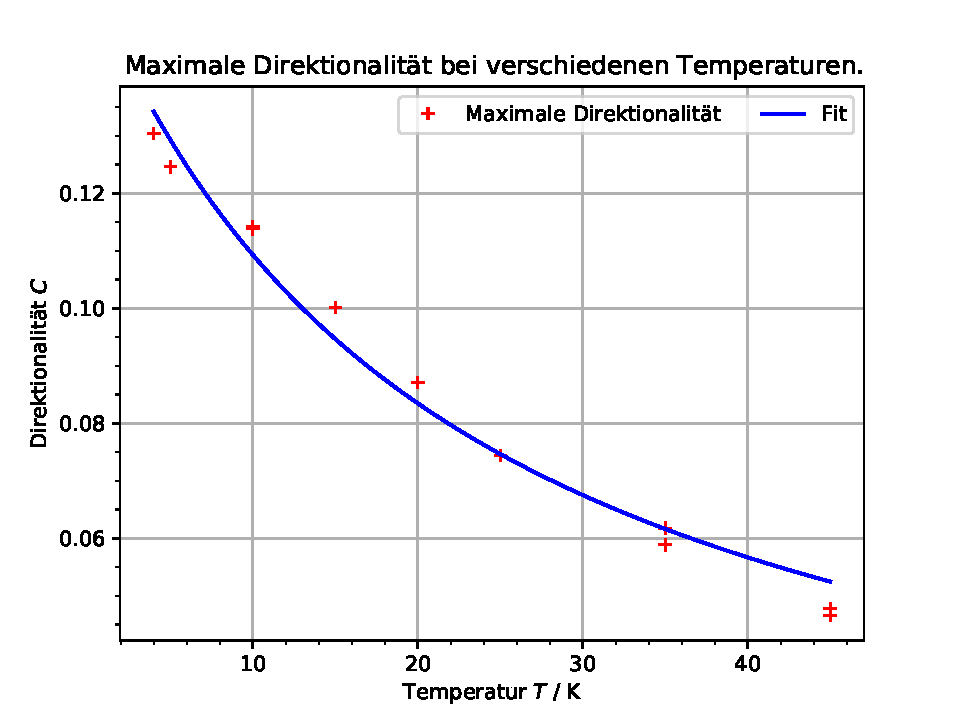
\includegraphics[scale=0.4]{images/Maximale_Rho_bei_Temperaturabhänigkeit.pdf}\\[-0.5\baselineskip]%
            }%
        \end{column}
    \end{columns}
\end{frame}

%\begin{frame}{Zusammenfassung}
%    \begin{itemize}
%        \item ja
%    \end{itemize}       
%\end{frame}

%\section{Ende}
\begin{frame}
    Danke für Ihre Aufmerksamkeit
\end{frame}


\begin{frame}{Backup}
    \centering
    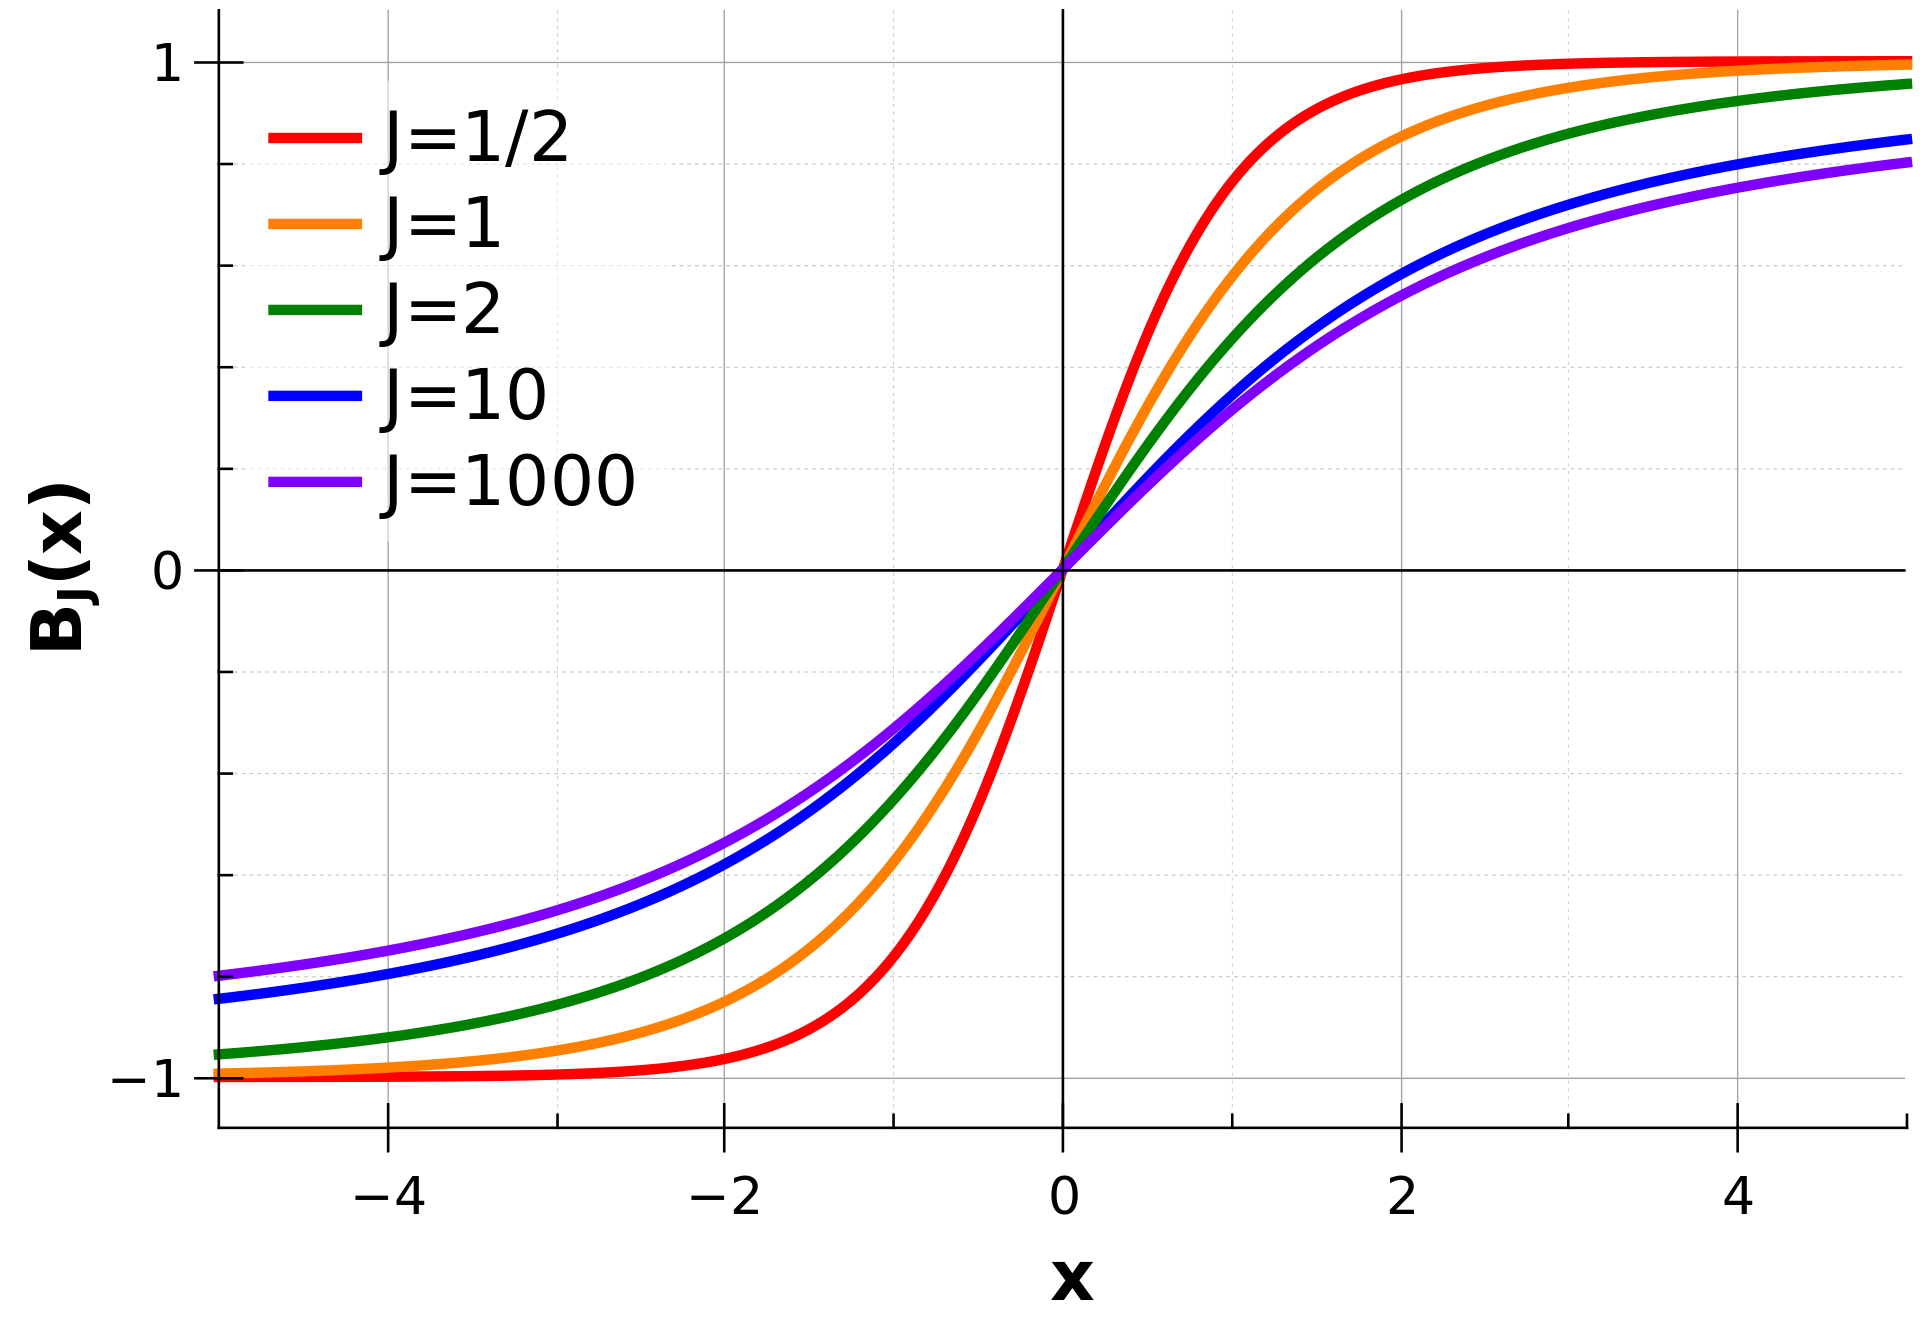
\includegraphics[scale=0.15]{images/b.png}\\[-0.5\baselineskip]
\end{frame}

\begin{frame}{Backup}
    \centering
    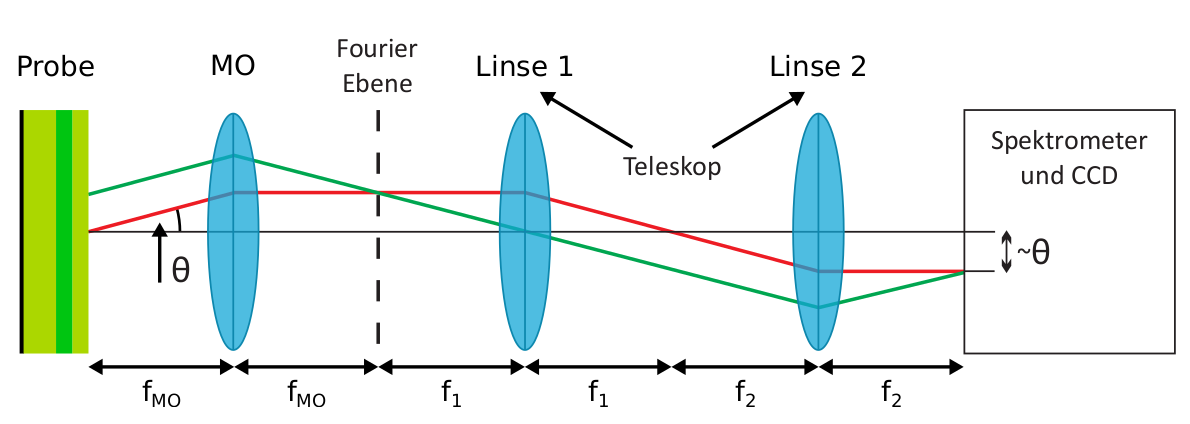
\includegraphics[scale=0.3]{images/lars.png}\\[-0.5\baselineskip]
\end{frame}

\end{document}
